\documentclass[10pt,a4paper]{article}
\usepackage[utf8]{inputenc}
\usepackage{amsmath}
\usepackage{amsfonts}
\usepackage{amssymb}
\usepackage{graphicx}
\usepackage{epstopdf}
\usepackage{inputenc}
\usepackage[a4paper, total={150mm,250mm}]{geometry}
\usepackage{graphicx}
\usepackage{hyperref}
\usepackage[dvipsnames, table]{xcolor}
\usepackage{subcaption}
\usepackage{fancybox, graphicx}
\usepackage{tikz}
\usepackage{array}
\usepackage{ulem}
\usepackage{enumitem}
\usetikzlibrary{shadows}
\usepackage{listings}
\usepackage{bm}
\usepackage{lmodern,textcomp}
\usepackage{listings}
%\usepackage[english]{babel}

\newcommand{\nline}{\\~\\}
\newcommand{\myparagraph}[1]{\paragraph{\normalsize{\textcolor{gray}{\uppercase{\textbf{#1}}}} }\mbox{} \vspace{0.5em}\\}
\usepackage{tikz}
\hypersetup{
    colorlinks=true, %set true if you want colored links
	linkcolor=black,
    linktoc=all,     %set to all if you want both sections and subsections linked 
    urlcolor=blue
}
\title{{\Huge\textbf{USDE  \\ Exam Preview Open Questions}}

\vspace{1em}
\normalsize{\textbf{Author}: \href{https://www.linkedin.com/in/simone-staffa-8b3b79158/}{Simone Staffa} \linebreak}

\vspace{1em}
\large \textcolor{red}{\textbf{Disclaimer!!} \\
\normalsize{This document is not intended to be a source of truth to prepare the exam. Therefore, I'm not responsible for wrong answers or errors reported here (even though I've done my best to provide valid material that regards all the topics that were spoken in the course). \\ Indeed all the questions answered here are taken from the \href{https://drive.google.com/file/d/1TWDK9OBrgVeqOfIp6SNplIrbFkuXcJ_9/view}{exam preview material} published on the \href{http://datascience.deib.polimi.it/course/unstructured-and-streaming-data-engineering/}{official site for the course (AA 2020/2021)}.}} \\
\vspace{30em}
\small{
Released with Beerware License, Rev. 42 (https://spdx.org/licenses/Beerware.html) \linebreak
“As long as you retain this notice you can do whatever you want with this stuff. If we meet some day, and you think this stuff is worth it, you can buy me a beer in return”}
}
\begin{document}
\maketitle
\clearpage
\tableofcontents
\clearpage
\section{Foundations}
\subsection{Data-driven decisions}
In many traditional organizations decisions are made by “questionable” methodologies such as \textbf{Highest Paid Person Opinion} (the boss decides) and \textbf{Flipism} (totally random). In the digital era one can dream of data-driven organization, taking decisions using data. According to McKinsey: \textit{“Decisions no longer have to be made in the dart or based on gut instinct; they can be based on evidence, experiments and more accurate forecasts.”}
\nline
Data-driven organizations:
\begin{itemize}
	\item \textbf{perform better}, since the data shows where they can streamline their process
	\item \textbf{are operationally more predictable}, with data insights fueling current and future decision making
	\item \textbf{are more profitable}, as constant improvements and better predictions help to outsmart competition and improve innovation
\end{itemize}

\subsection{4 Vs of Big Data}
BigData is a term that describes the large volume of data - both structured and unstructured - that inundates a business on a day-to-day-basis. IBM data scientists break big data into four dimensions:
\begin{itemize}
	\item \textbf{Volume} (data at scale): volume is increasing, we have more and more data
	\item \textbf{Variety} (data in many form): structured, unstructured or semi-structured
	\item \textbf{Velocity} (data in motion): analysis of streaming data to enable decision within fractions of a second (real-time decision and data analysis while data are coming)
	\item \textbf{Veracity} (data uncertainty): managing the reliability and predictability of inherently imprecise data type (the same data could be good or not good according to the different purpose for which it is used)
\end{itemize}
\subsection{"oil" metaphor for Big Data, Data Science and Data Engineering}
\myparagraph{"oil" metaphor for Big Data}
\textit{“Data is just like crude oil. It’s valuable, but if unrefined it cannot really be used. It has to be changed into gas, plastic, chemicals, etc to create a valuable entity that drives profitable activity; so data must be broken down and analyzed for it to have value.”}
\nline
Recently it became evident that data indeed represents incredible economic and societal value. Using the metaphor “data=oil” we can definitely see similarities:
\begin{itemize}
	\item \textbf{Exploration}: just like we need to find oil, we need to locate relevant data before we can extract it
	\item \textbf{Extraction}: after locating the data (oil), we need to extract it
	\item \textbf{Transform}: we then need to clean, filter and aggregate data (oil)
	\item \textbf{Storage}: data (oil) needs to be stored and this may be challenging if it is huge
	\item \textbf{Transport}: getting the data (oil) to the right person, organization or software tool (to the petrol station)
	\item \textbf{Usage}: while driving a car one consumes oil. Similarly, providing analysis results requires data
\end{itemize}
So the different stages from exploring crude oil to using it to drive a car also apply to data science. 

\pagebreak However, there are some important differences between data and oil:
\begin{itemize}
	\item \textbf{Copying data is relatively easy and cheap}. While it is impossible to simply copy a product like oil.
	\item \textbf{Data is specific, i.e., it relates to a specific event, object, and/or period}. Different data elements are not exchangeable. When going to a petrol station, this is very different; drops of oil are not preallocated to a specific car on a specific day.
	\item Typically, \textbf{data storage and transport are cheap} (unless the data is really Big Data). In a communication network, data may travel (almost) at the speed of light and storage costs are much lower than the storage costs of oil.
\end{itemize}
\myparagraph{Data Science vs. Data Engineering}
Data science is the activity of refining crude oil. Data science, in the end, creates value. We spend money to find and extract crude oil, as we spend money to collect and prepare data. While when we refine data (cleaning and analysis) we create value.
\nline
\textbf{Data Science is the art of discovering what we don’t know from data. It allows obtaining predictive and actionable insights from data.} Indeed, Data Scientists are a new breed of analytical data expert who have the technical skills to solve complex problems. They’re part mathematician, part computer scientist and part trend-spotter. 
\nline
Following the crude oil example, data engineers build “the refinery”. \textbf{A data engineer is a specialist that maintain data and models available and usable by others (i.e., data scientists).} According to Google, a professional data engineer enables data-driven decision making by collecting, transforming and publishing data. He should be also able to leverage, deploy and continuously train pre-existing machine learning problems.
\subsection{4 paradigmatic shifts to solve old problems in new ways}
\myparagraph{Selection of Data}
\textcolor{blue}{Collect perfect data vs. Collect huge amount of imperfect data}
\nline
Traditionally when you have infinite analytical capabilities, you use a good statistical sample of the entire space of data. It takes time to design an experiment with a significant sample. \\
\textbf{The innovative approach is enabled by the possibility to tame the data volume. Doesn’t matter how much data, it fits somewhere. Instead of defining which data you want first, you explore your data searching for useful information.}
\nline
\uline{Example:}
The largest good transportation company in the USA on railways. \\ The big problem for anybody that is running trains, is that, if you have an accident it takes time to restore the line and in the meantime, you lose a business opportunity. 
The traditional way sends around expensive machines that can do extreme precise measurements. If the measurements are not clear enough, people will measure it manually (collecting perfect data for the work that they need to do). \\
The innovative way consists in using a complex sensor that measures things with high precision. A huge amount of data is collected. This data will lead to the same measurements and the same frequency as the traditional system. Collecting a huge amount of data that will cost very little, and in the end you can obtainthe same results. This is enabled by the central limit theorem. Large enough dataset at a certain point reaches the same result, since the sample means of a sufficiently large dataset is approximately normally distributed. 
\pagebreak
\myparagraph{Data-driven exploration}
\textcolor{blue}{Hypotesis and Tests vs. Explore data and get insights}
\nline
The traditional business intelligence approach starts with a hypothesis and tests against selected data. You guess that something can be true, and you go to the data warehouse writing a query, and checking if your hypothesis is true. \\
\textbf{The innovative approach is one of unstructured machine learning. Explore data and look for patterns getting insights. Building models and describing statistical phenomena being able to do it at scale. }\nline
\uline{Example:} \\
In a supermarket business, take all the receipts and look for all the pairs of goods that are purchased within the same receipt. Then compute the probability of pairing two products in the same receipt. You can discover patterns like a client that buys beers has a good chance of buying huggies.

\myparagraph{Reduce the effort required to leverage data}
\textcolor{blue}{Combine data after a long preparation vs. Combine messy data that you cleanse when needed}
\nline
The traditional approach, when you have to take some data and bring them together, you make sure that data is clean and collected in the proper way which makes sense to combine them. \\
\textbf{The innovative approach collects and combines data without cleaning it first. You just collect a large amount of messy data that you cleanse when needed.} \nline
\uline{Example:}
\begin{itemize}
	\item \textbf{Traditional:} I do statistical samples and then I have techniques that tell me if they can be merged. Hard to scale.
	\item \textbf{Innovative}: if you collect a lot of data, there will be for sure some statistical samples that can be merged.
\end{itemize}

\myparagraph{Leverage data as it is captured}
\textcolor{blue}{Analyse data aftern it's been processed vs. Analyse data as it is generated}
\nline
Traditional approach analyses data after it’s been processed and landed in a warehouse or mart. \\
\textbf{Innovative approach analyse data in motion as it’s generated, in real-time.} \nline
\uline{Example:} \\
Machine learning and deep learning: real-time data analysis and image detection, like a car that tags each object it sees during the street.
Algorithms that take decisions in real-time (in trading sell or buy in 10ms) 
\subsection{Schema on Write vs. Schema on Read}
One of the main paradigmatic shifts introduced by Big Data consists in the transition from schema on write to schema on read. \\
\textbf{Schema on write} characterizes the rigid and traditional relational databases in which a complex schema is applied after a long lasting design phase. Using this strategy, we collect the data from different sources, ensuring that it is compatible with our schema and then we make analysis on that. \\
\textbf{Schema on read} follows a schema-less approach in which we collect and load data first and ask questions/queries later. All data are kept and the minimal schema for an analysis is applied only when needed. New analysis can then be introduced at any point in time.
\pagebreak
\subsection{Horizontal vs. Vertical Scalability}
Scalability means the ability to expand the computer resources to handle the exponential growth   of work. Database scalability means the ability of a system’s database to scale up or down as per the requirement. If the database isn’t scalable, then the processes can slow down or even fail which can be quite detrimental to the business operations. Further, it enables the database to grow to a larger size to support more transactions as the volume of business and/or customer count grows.
\nline
There are two types of scalability:
\begin{itemize}
	\item \textbf{traditional SQL system scale vertically}: when the machines, where the SQL system runs, no longer performs as required, the solution is to buy a better machine (with more RAM, more cores and more disk)
	\item \textbf{Big data solutions scale horizontally}: when the machines, where the big data solution runs, no longer performs as required, the solution is to add another machine.
\end{itemize}
Of course there are scenarios in which scaling vertically is convenient w.r.t. to scaling horizontally (and vice versa). In general, as data size grows up to a certain limit, big data solutions (and horizontal scalability) are more convenient. While traditional relational databases (and vertical scalability) are more convenient with smaller datasets. The breakeven point in which big data solutions are more convenient w.r.t. to traditional relational databases is becoming smaller every year. For example, now the breakeven point between the two technologies is around 10TBs of data, after which traditional solutions’ cost grows exponentially, while big data solutions’ cost grows linearly.
\subsection{Data partitioning/sharding and Replication}
\myparagraph{Sharding vs. Partitioning}
\textbf{Sharding is the practice of optimizing database management systems by separating the rows or columns of a larger database table into multiple smaller tables.} The new tables are called “shards” (or partitions), and each new table either has the same schema but unique rows (as is the case for “horizontal sharding”) or has a schema that is a proper subset of the original table’s schema (as is the case for “vertical sharding”).
\nline
Sharding is a common concept in scalable database architectures. By sharding a larger table, you can store the new chunks of data, called logical shards, across multiple nodes to achieve horizontal scalability and improved performance. Once the logical shard is stored on another node, it is referred to as a physical shard.
\nline
\textbf{Sharding and partitioning are both about breaking up a large data set into smaller subsets. The difference is that sharding implies the data is spread across multiple computers while partitioning does not.} \uline{Partitioning is about grouping subsets of data within a single database instance.} In many cases, the terms sharding and partitioning are even used synonymously, especially when preceded by the terms “horizontal” and “vertical.” Thus, “horizontal sharding” and “horizontal partitioning” can mean the same thing.
\pagebreak
\myparagraph{Replication}
\textbf{Data replication is the process of making multiple copies of data and storing them at different locations to improve their overall accessibility across a network.} Similar to data mirroring, data replication can be applied to both individual computers and servers. The data replicas can be stored within the same system, on-site and off-site hosts, and cloud-based hosts.
\nline
Although data replication can be demanding in terms of cost, computational, and storage requirements, businesses widely use this database management technique to achieve one or more of the following goals:
\begin{itemize}
	\item \textbf{Improve the availability of data}: once a node in the distributed system is down, data can still be access from another working node
	\item \textbf{Enhance server performance}: data replication reduces the load on the primary server by dispersing it among other nodes in the distributed system, thereby improving network performance
	\item \textbf{Accomplish disaster recovery}:  Data replication facilitates the recovery of data which is lost or corrupted by maintaining accurate backups at well-monitored locations, thereby contributing to enhanced data protection.
\end{itemize}
 \subsection{Logical Architecture of a Big Data Platform}
 The logical architecture isolates several logic areas and several processes that somehow move data between these areas. \textbf{Data ingestion} is the process that brings the data from outside into an area where you can land anything in any format and any schema, you just place raw things that stays for a while (\textbf{Raw Big Data Landing Zone}). If you are interested in this raw data, you move it to the \textbf{Big Data Long Term Storage Zone} through the \textbf{Data Wrangling} process. Here you try at least to put data in formats (normally columnar formats) because you tend to do analytics. By the way you are not providing an integrated schema, just you put data in a minimal format that facilitates the query process. Then with ETL (extract-transform-load) processes you transform this data in a specific schema, moving data to the \textbf{Consumption zones}. In these places you are providing specific schemas to allow the use of data from business intelligence applications.
\nline
Big Data introduced a paradigmatic shift from schema-on-write to schema-on-read. 
Schema-on-write is the rigid and traditional strategy (relational data) in which a complex schema is applied after a long lasting discussion (long design phase). Here we collect the data from different sources, ensuring that it is compatible with our schema and then we make analysis on that.
Schema-on-read is a schema-less approach (unstructured data) in which we collect and load data first and perform queries later. All data are kept and the minimal schema for analysis is applied only when needed. New analysis can be introduced at any point in time. Here we have massive data-writing and not schema related, and we can perform analysis on small pieces of data using a minimal schema (not a general schema for the entire business). \\
This strategy (schema-on-read) moves us towards the concept of data lake. A data lake is a sort of repository of data, that is raw container of any kind of data. You may have many different flows of data coming in the repository, that could feature both structured and unstructured data (raw data, text, documents, multimedia). You know that you have one reference place for the entire organization for containing all the data of the organization. Past approaches could have different divisions of an organization dealing and managing with different data stored in different repositories. At any time you can have an outgoing flow of data that can be used for analysis. \\
Weaknesses of this approach:
\begin{itemize}
	\item It’s harder to select the right chunk of data that you are looking for in your analysis.
	\item Scalability problem: since this lake can become bigger and bigger, you need to ensure to have the right resources to support it.
	\item How do we connect to the incoming data? If we just throw in this data in a completely messy way, the result is not a lake. You end up with something totally useless.
\end{itemize}
In reality things are not so naive and messy. The data lake process is a little bit more complex. We still support many different kinds of data (structured and unstructured data). This kind of data goes through a set of steps in a process that from a very raw and diverse and heterogeneous format tries to make things a little more accessible and usable in the future.
\begin{enumerate}
	\item First you just ingest data and build a catalog.
	\item In the second step, where the data is still raw, at least you add some metadata (e.g., who is the owner, what is describing etc.)
	\item Then, you run some kind of quality check and validation. The data you get could be noisy, messy or dirty, so you need some quality check. Towards big data, data becomes bigger but also messy. The probability of having noise is increasing.
	\item Now we have the problem of enrichment of the data. Because the data we get may be very narrow or granular, and so we need to empower it with integration with other data.
	\item In the end, when someone wants to read some output, we will build a data extractor, analyser and visualizer to show data.
\end{enumerate}

\pagebreak

\section{NoSQL \& Data Models}
\subsection{Features and differences between the presented models}
\textbf{“NoSQL” generally refers to any DBMS that doesn’t employ the relational model.} The data models presented in class are: Key-value store (Redis, Memcached), Columnar database (Cassandra), Document store (MongoDB), Graph database (Neo4j).
\myparagraph{Key-Value databases}
\textbf{Key-value databases work by storing dictionaries or hash tables}, which are a collection of key-value pairs in which a key serves as a unique identifier to retrieve an associated value. Values can be anything from simple objects, like integers or strings, to more complex objects, like JSON structures. A key-value database treats any data held within it as an opaque blob; it’s up to the application to understand how it’s structured. \\
Key-value databases are often described as \textbf{highly performant, efficient, and scalable. Common use cases for key-value databases are caching, message queuing, and session management.}
\nline
\uline{Example:}
\textbf{Redis} is an in-memory data store used as a database, cache, or message broker. It supports a variety of data structures, ranging from strings to bitmaps, streams and spatial indexes.

\myparagraph{Columnar Databases}
Columnar databases are database systems that store data in columns. \textbf{The goal of a columnar database is to efficiently write and read data to and from hard disk storage in order to speed up the time it takes to return a query.} In a columnar database, all the column 1 values are physically together, followed by all the column 2 values, etc. The data is stored in record order, so the 100th entry for column 1 and the 100th entry for column 2 belong to the same input record. This design allows queries to only read the columns they need, rather than having to read every row in a table and discard unneeded data after it’s been stored in memory. Because the data in each column is of the same type, they allow for various storage optimizations, since data can be highly compressed. The most used compression technique is run-length encoding, which allows minimizing the amount of space taken up by a single column, speeding up reads since queries need to go over fewer rows.		
\nline
\textbf{In terms of performance, there’s a breakeven point in which relational databases are convenient w.r.t. columnar databases since traditional queries always read all the rows.} If columnar databases are required to read too much data, after a certain point, they are then outperformed by relational databases (whose read performance is constant).
\nline
Columnar databases have become widely used for \textbf{data analytics} since the columnar data model lends itself well to fast query processing. They’re also seen as advantageous in cases where an application needs to \textbf{frequently perform aggregate functions}.
More in general, columnar databases excel at:
\begin{itemize}
	\item \textbf{Queries that involve only a few columns}
	\item \textbf{Aggregation queries against vast amount of data}
	\item \textbf{Column-wise compression}
\end{itemize}
\uline{Example}: \textbf{Cassandra} is a highly scalable, high-performance distributed database designed to handle large amounts of data across many commodity servers, providing high availability with no single point of failure
\pagebreak
\myparagraph{Document-oriented databases}
\textbf{Document-oriented databases are NoSQL databases that store data in the form of documents.} \textbf{Document stores are a type of key-value store}: each document has a unique identifier - its key - and the document itself serves as the value. 		\\
\uline{The main difference between these two models is that, in a key-value database, the data is treated as opaque} and the database doesn’t know or care about the data held within it; it’s up to the application to understand what data is stored. \textbf{In a document store}, however, \textbf{each document contains some kind of metadata that provides a degree of structure to the data}. Moreover, document stores often come with an API or query language that allows users to retrieve documents based on the metadata they contain. They also allow for complex data structures, as you can nest documents with other documents. \\
\textbf{Document stores typically store data as JSON or XML documents.} \\
Thanks to their flexible schema, they’ve found regular use in \textbf{e-commerce, blogging, and analytics platforms}, as well as content management systems. Document stores are considered \textbf{highly scalable}, with \textbf{sharding being a common horizontal scaling strategy}. They are also excellent for \textbf{keeping large amounts of unrelated, complex information that varies in structure.}
\nline
Key features document stores:
\begin{itemize}
	\item \textbf{Flexible schema}: structure of individual documents does not have to be consistent; easier to integrate new information
	\item \textbf{Better read performance}: information is contained in a single location (a document), no relations needed to access nested data
\end{itemize}
\uline{Example:} \textbf{MongoDB} is a general-purpose, distributed document store, definitely the world’s most widely used document-oriented database.

\myparagraph{Graph Databases}
\textbf{Graph databases can be thought of as a subcategory of the document store model, in that they store data in documents and don’t insist that data adhere to a predefined schema.} The difference though is that \uline{graph databases add an extra layer to the document model by highlighting the relationships between individual documents}. \nline
To better grasp the concept of graph databases, it’s important to understand the following terms:
\begin{itemize}
	\item \textbf{Node}: a node is a representation of an individual entity tracked by a graph database. It is more or less equivalent to the concept of a record or row in a relational database or a document in a document store. For example, in a graph database of music recording artists, a node might represent a single performer or a band.
	\item \textbf{Property}: a property is relevant information related to individual nodes. Building on our recording artist example, some properties might be “vocalist”, “jazz”, or “platinum-selling artist”, depending on what information is relevant to the database.
	\item \textbf{Edge}: also known as a relationship, an edge is the representation of how two nodes are related and is a key concept of graph databases. Edges can be directed or undirected as in traditional graph data structures.
\end{itemize}
Certain operations are much simpler to perform using graph databases because of how they link and group related pieces of information. \textbf{These databases are commonly used in cases where it’s crucial to be able to gain insights from the relationships between data points} or in applications where the information available to end-users is determined by their connections to others, \textbf{as in a social network}.
\nline
The main advantages of graph databases are on:
\begin{itemize}
	\item \textbf{Performance}: in contrast to relational databases, where join-intensive query performance deteriorates as the dataset gets bigger, with a graph database performance tends to remain relatively constant, even as the dataset grows. This is because queries are localized to a portion of the graph.
	\item \textbf{Flexibility}: As developers and architects, we want to connect data as the domain dictates, thereby allowing structure and schema to emerge in tandem with our growing understanding of the problem space, rather than being imposed upfront. Graph databases address this need directly.
	\item \textbf{Agility}: we want to be able to evolve our data model in step with the rest of our application. The schema-free nature of graph data model, coupled with the testable nature of a graph database’s API and query language empower us to evolve an application in a controlled manner.
\end{itemize}
\uline{Example:} \textbf{Neo4j} is an ACID-compliant DBMS with native graph storage and processing. It is the most popular graph database in the world.
\subsection{ACID vs. BASE}
\textbf{ACID and BASE are two consistency models for data in transactions.}
\nline
\textbf{ACID is the consistency model mainly used by traditional relational databases}, for this reason, has been the standard for some time. The key ACID guarantee is that it provides a safe environment in which to operate on your data. \\
The ACID acronym stands for:
\begin{itemize}
	\item \textbf{Atomicity}: all operations in a transaction succeed or every operation is rolled back
	\item \textbf{Consistency}: the transaction satisfies the integrity of constraints on data. As a consequence, if the initial state is consistent, then the final state is also consistent
	\item \textbf{Isolation}: a transaction is not affected by the behaviour of other, concurrent transactions
	\item \textbf{Durability}: the effect of a transaction that has successfully committed will last “forever” independently of any system fault
\end{itemize}
By the way, from many domains and use cases, ACID transactions are far more pessimistic than the domain actually requires. In the NoSQL database world, ACID transactions are less fashionable as some databases have loosened the requirements for immediate consistency, data freshness and accuracy in order to gain other benefits, like scale and resilience. \\
The BASE acronym stands for:
\begin{itemize}
	\item \textbf{Basic Availability}: fulfil requests, even in partial consistency. Basic functionalities are always provided
	\item \textbf{Soft State}: abandon the consistency requirements of the ACID model pretty much completely
	\item \textbf{Eventual Consistency}: at some point in the future, data will converge to a consistent state. Delayed consistency, as opposed to immediate consistency of the ACID properties.
\end{itemize}
In general, \textbf{BASE properties are much looser than ACID guarantees}, but there isn’t a direct one-to-one mapping between the two consistency models. \textbf{A BASE datastore values availability} (since that’s important for scale), \textbf{but it doesn’t offer guaranteed consistency of replicated data at write time}. Overall, \textbf{the BASE consistency model provides a less strict guarantee than ACID}.
\subsection{CAP Theorem}
The CAP theorem states that it is impossible for a distributed system to simultaneously provide all three of the following guarantees:
\begin{itemize}
	\item \textbf{Consistency} (C): all nodes see the same data at the same time 
	\item \textbf{Availability} (A): node failures do not prevent other survivors from continuing to operate
	\item \textbf{Partition Tolerance} (P): the system continues to operate despite arbitrary partitioning due to network failures (e.g., message loss)
\end{itemize}
\textbf{A distributed system can satisfy any two of these guarantees at the same time but not all three.} In a distributed system, a network partition is inevitable by definition. We can’t avoid dealing with partition tolerance, we need to cover that. Indeed, failures can and will occur in a networked system. Then the only option left is choosing between Consistency and Availability. This because Consistency+Availability does not make any sense because is what traditional centralized databases are guaranteeing. In the end, either we choose A+P or C+P.  \\
By the way, \uline{Consistency and Availability should not be considered as mutually exclusive}. Is possible to guarantee a partial accommodation of both. We can do some trade-off analysis, knowing that, for example, consistency is preferred in banking applications where the transactions of money must be consistent at any time, while availability is preferred in social networks where some user content can even be presented in an outdated version.
\subsection{Neo4J}
\textbf{Neo4j is the most popular graph database}. It is \textbf{schema free}, meaning that data does not have to adhere to any structure/convention. Moreover \textbf{it enforces the ACID consistency model}. \\ 
\uline{Neo4j is meant to be an operational DB, not specifically for analytics}. Thus, it is efficient on nodes and patterns, while is not so efficient in whole-graph analysis. The data model of Neo4j is composed of: nodes (with labels and attributes), edges and indexes.
\nline
Queries on Neo4j can be written using Cypher, an expressing graph database query language. This language enables the user to ask the database to find data that matches a specific pattern. Among the most used clauses we have: 
\begin{itemize}
	\item \textbf{Match}: used to specify a pattern to be matched (in a way similar to ASCII art)
	\item \textbf{Where}: provides criteria for filtering pattern matching results
\end{itemize}

\subsection{Redis}
\textbf{Redis is an advanced key-value store}, where keys can contain data structures such as strings, hashes, lists, sets and sorted sets. It supports a set of atomic operations on these data types. Redis is a different evolution path in the key-value databases where values are complex data types that are closely related to fundamental data structures and are exposed to the programmer as such, without additional abstraction layers. \\
It can be used as:
\begin{itemize}
	\item \textbf{Database}: Redis can persist data on disk
	\item \textbf{Caching Layer}: Redis is fast
	\item \textbf{Message broker}: Redis is not only a key-value store
\end{itemize}
\uline{Redis is not a replacement for Relational Databases nor Document stores. It might be used complementary to a SQL relational store, and/or NoSQL document store.} Even when Redis offers configurable mechanisms for persistency, increased persistency will tend to increase latency and decrease throughput.
\textbf{Regarding the CAP theorem, Redis enforces Consistency and Partition Tolerance.}
\nline
When to use Redis:
\begin{itemize}
	\item Speed is critical
	\item Dataset can fit in memory
	\item Dataset is not critical
\end{itemize}
Redis has offers different option for scaling purposes:
\begin{itemize}
	\item \textbf{Persistence}: it can persist data on disk in two modes:
	\begin{itemize}
		\item saving memory snapshot on disk (like a backup)
		\item storing in append mode the evolution of data
	\end{itemize}

	\item \textbf{Replications}: a Redis instance known as the master ensures that one or more instances known as the slaves become exact copies of the master. Clients can connect to the master or to the slaves. Slaves are read-only by default, while master allows both read and write operations.
	\item \textbf{Partitioning}: we need to deal with data separation, breaking up data and distributing it across different hosts in a cluster. It can be implemented in different layers:
	\begin{itemize}
		\item \uline{Client}: partitioning on client-side
		\item \uline{Proxy}: an extra layer that proxies all Redis queries and perform partitioning
		\item \uline{Query Router}: instances will make sure to forward the query to the right code
	\end{itemize}

	\item \textbf{Failover}: replace possible master that is broken with a slave
	\begin{itemize}
		\item Manual
		\item Automatic with Redis Sentinel
		\item Automatic with Redis Cluster
	\end{itemize}

\end{itemize}
Redis offers 4 topologies, with different advantages:
\begin{itemize}
	\item \textbf{Standalone} (optional data redundancy on client-side)
	\item \textbf{Sentinel} (automatic failover)
	\item \textbf{Twemproxy} (distributed data)
	\item \textbf{Cluster} (automatic failover and distributed data)
\end{itemize}

\subsection{Cassandra}
Cassandra is a columnar database which was originally designed at Facebook and then open-sourced. It can be considered a hybrid of Google’s Bigtable (columnar) and Amazon’s Dynamo (key-value). \\
Cassandra properties:
\begin{itemize}
	\item \textbf{highly available}
	\item \textbf{fault tolerant}
	\item \textbf{tuneably consistent}: allows to have some levels of consistency which can be tuned dynamically (trade-off with performance)
	\item \textbf{very fast writes}
	\item linear, elastic scalability
	\item decentralized/symmetric (no master/slave) -> ring topology
	\item automatic provisioning of new nodes 
	\item \textbf{constant read complexity} $\rightarrow$ O(1) DHT key-based query
\end{itemize}
\textbf{Cassandra Cluster uses a gossip protocol to know which nodes are online and working.} Gossip is a peer-to-peer communication protocol in which nodes periodically exchange state information about themselves and about other nodes they know about. In the end all nodes quickly learn about all other nodes in the cluster.
\nline
As said, \textbf{Cassandra is fault-tolerant}. It places replicas of data on different nodes based on these two factors:
\begin{itemize}
	\item \textbf{Replication Strategy}: where to place the next replica
	\item \textbf{Replication Factor}: total number of replicas placed on different nodes
\end{itemize}
$ReplicationFactor = 1$ means that there is only a single copy of data in the cluster, while $ReplicationFactor = 3$ means that there are three copies of the data on three different nodes. \textbf{For ensuring there is no single point of failure, replication factor must be three}. 

\pagebreak
There are two kinds of replication strategies in Cassandra:
\begin{itemize}
	\item \textbf{Simple Strategy}: used when you have just one data center. It places the first replica on the node selected by the partitioner. After that, remaining replicas are placed in clockwise direction in the Node ring.
	\item \textbf{Network Topology Strategy}: is used when you have multiple data centers. This strategy places replicas in the same datacenter by walking the ring clockwise until reaching the first node in another rack. NetworkTopologyStrategy attempts to place replicas on distinct racks because nodes in the same rack (or similar physical grouping) often fail at the same time due to power, cooling, or network issues.
\end{itemize}
\textbf{Regarding the CAP theorem, Cassandra concentrates on Availability and Partition tolerance.} Nonetheless, it has some levels of consistency. \\
The Cassandra consistency level is defined as the minimum number of Cassandra nodes that must acknowledge a read or write operation before the operation can be considered successful. \textbf{Consistency level is tuneable in the sense that the user can configure the minimum number of nodes required to reach the quorum} (from one to all).
\nline
Keyspace is the outermost container for data in Cassandra. The basic attributes of a Keyspace are: 
\begin{itemize}
	\item \textbf{Replication factor}: the number of machines in the cluster that will receive copies of the same data
	\item \textbf{Replication strategy}: the strategy to place replicas in the ring
	\item \textbf{Column families}: a container of a collection of rows, each row contains ordered columns. Column families represent the structure of your data. Each keyspace has at least one and often many column families.
\end{itemize}
A\textbf{ column family} is a container for an ordered collection of rows. Each row, in turn, is an ordered collection of columns. Each column consists of a name (key), a value and a clock timestamp which indicates the update time. \textbf{Column families are sparse tables} in the sense that not all the records (rows) must have a value for all the columns. Some rows could contain only a few columns, while some others may contain all of them.  \\
As mentioned earlier, \textbf{Cassandra is a hybrid key-value based and column based database.} Indeed, we can consider each row as a key which points to a set of columns (the value). Somehow we could say that Cassandra is a key-value based database in which the value is internally structured as columns.
\textbf{Super columns} group columns under a common name.
\nline
Cassandra is a good fit when:
\begin{itemize}
	\item You need really fast writes (and reads)
	\item You need durability
	\item You have lots of data ($>$ GBs)
	\item You need a fluid data structure
\end{itemize}

\subsection{MongoDB}
\textbf{MongoDB is an open source and document-oriented database}. \textbf{It stores data in JSON-like documents}. It is designed with both scalability and developer agility in mind. It allows \textbf{dynamic schemas} and \textbf{dynamic data sharding}.
\nline
The major and very common problem with a growing web application is scaling. To overcome this, MongoDB has come up with a \textbf{Sharding} feature. It is one of the greatest key features of MongoDB. Sharding is a method for distributing data across multiple machines.
\uline{Sharding makes it possible to provide horizontal scalability}. Each shard holds a portion of the data and functions as a separate database. The collection of several shards together is what forms a single logical database.
\nline
MongoDB is a \textbf{schema-less database} and, because of it, is much more flexible than traditional database tables. The benefit is the lack of setup and the reduced friction with OOP. So, in order to save an object, you just have to serialize it to JSON and send it to MongoDB. There is no need for type mapping which removes an additional burden.
\nline
\textbf{Indexes are created to improve the performance of searches}. The good thing is that any field in a MongoDB document can be indexed with primary and secondary indices. It enables the database engine to efficiently resolve queries.
\nline
MongoDB provides \textbf{replication} features by distributing data across different machines. It can have one primary node and one or more secondary nodes. This typology is known as replica set. Replica set is like master-slave replication. A master can perform reads and writes while a Slave copies data from the master and can only be used for reads or back up (not writes). \\ Another robust feature of the MongoDB replica set is its \textbf{automatic failover}.
When one of the set members can’t reach the primary instance for more than 10 seconds, the replica set will automatically elect and promote a secondary instance as the new primary.
\nline
Regarding the CAP theorem, \textbf{MongoDB concentrates on Consistency and Partition Tolerance}. 
\begin{itemize}
	\item It ensures that all replicas contain the same version of the data at any time.
	\item It ensures that system remains operational on system split (multiple entry points)
\end{itemize}
For what concerns Availability, MongoDB’s replication strategy allows the system to remain operational even with failing nodes.

\pagebreak

\section{Streaming Data Engineering}
\subsection{Throughput vs. Latency vs. Message Size}
How do we move data between zones in the logical architecture of a big data platform? What’s the solution space in trying to solve this problem?
\\
To answer these questions, we have few dimensions that we have to think about: throughput, latency and message size. These dimensions matter when you want to understand how the solution space is organized.
\nline
Throughput indicates how much data we are able to ingest in a given time interval. It is the main performance indicator that we aim to optimize. Latency is the total time that we need to transport a message. Message size is the size of the messages that we transport. 
Actually, our aim is to maximize throughput and minimize latency. By the way, this is not so easy. Indeed, there’s a trade-off between latency and throughput: high latency corresponds to high throughput while low latency corresponds to low throughput. 

\subsection{Ultra-bulk vs. Batch vs. Continuous Data Ingestion \& Preparation}
When dealing with latency-throughput trade-off there are at least three cases that are along a continuum.
\begin{itemize}
	\item The \textbf{Ultra Bulk} case is characterized by high throughput and high latency. We are talking about latency in terms of days and message size in terms of petabytes. One and only big transfer of data. \\
\uline{Example}:
imagine that you have a data warehouse with petabytes of data and you would like to transfer this data on the cloud once for all. There are different solutions that you can use such as Ultra Wide Band (2,5 Gbps $\rightarrow$ 37 days), Infinity Band (54 Gbps $\rightarrow$ 1,7 days) and Google Transfer Appliance (2 days)
	\item The \textbf{Continuous} case is characterized by low throughput and low latency. We are talking about latency in terms of ms and message size in terms of kilobytes. \\
\uline{Example}:
a real time inventory for a company that has many physical shops and also sells online through an e-commerce platform. You can use Kafka to build an event system that captures all the product purchases and updates the stock correspondingly. A lot of small messages running in the system at any time. 
	\item The \textbf{Batch} case has a balanced throughput-latency trade-off. \\
\uline{Example}:
Tracking customer journeys 360° by attaching a Change Data Capture process to all the different applications in your system. Then store the changes in a temporary blob storage. Finally each hour push the changes to a data warehouse that you use for analytics. Balanced size of messages and latency.
\end{itemize}

 \subsection{Batch Approach: Append vs. Compaction Mode}
 \myparagraph{Batch Approach}
 In a distributed system dealing with Big Data (where complex failure patterns can happen) we usually apply Write Once, Read many principles.
 \begin{itemize}
 	\item Allows reliable and parallel writing
 	\item Simplifies data coherency issues
 	\item Enables high throughput data access

 \end{itemize}
 As a consequence
\begin{itemize}
	\item All data are kept in immutable files
	\item Append-only operations are allowed
\end{itemize}
\pagebreak
The Batch approach allows for two options:
\begin{itemize}
	\item the \textbf{OVERWRITE} option in which the ingested table is overwritten each time, and a new view is used to map all the ingested table to a common structure
	\item the \textbf{BATCH} option in which 
	\begin{itemize}
	\item the first time a file is ingested \& wrangled and an history table is created
	\item the next times there are two options
	\begin{itemize}
			\item \textbf{APPEND MODE}: this approach consists in appending batches at the end of the history table, treating changes as inserts at a given timestamp
		\item \textbf{COMPACTION MODE}: this approach maintains only the most recent version for each key, treating changes as updates
		\end{itemize}
\end{itemize}
\end{itemize}

\myparagraph{Append vs. Compaction Mode}
\textbf{Append Mode Pros}
\begin{itemize}
	\item minimal ingestion \& wrangling cost
	\item the version of data in any point in time can be rebuilt
\end{itemize}
\textbf{Append Mode Cons}:
\begin{itemize}
	\item it requires more space than keeping only the most recent version
	\item if multiple ETLs access the same data, the same computation may be repeated
\end{itemize}
\textbf{Compaction Mode Pros:}
\begin{itemize}
	\item it requires less space than keeping all version as in append only mode
	\item multiple ETLs can access the same data without additional computation
\end{itemize}
\textbf{Compaction Mode Cons:}
\begin{itemize}
	\item it requires more computation that ingestion and wrangling in append only mode
	\item only the most recent version of data is available, build version in arbitrary points in time is impossible
\end{itemize}

\subsection{Continuous Approach}
\subsubsection{DSMS}
\myparagraph{Semantics}
Data Stream Management Systems (DSMS) are used to manage streams of data. Data streams are unbounded sequences of time-varying data elements. They represent an almost continuous flow of information, with the recent information being more relevant as it describes the current state of a dynamic system. \\
The nature of streams requires a paradigmatic change \textbf{from persistent data} (one time semantics) \textbf{to transient data} (continuous data flow, with static queries). Indeed, continuous queries can be registered over streams that are observed through “windows” (time intervals in which we are interested in analysing data).

\myparagraph{Time representations (Causal, Absolute \& Interval)} 
The time model defines the relationship between information items and passing of time. It allows an Information Flow Processing system to associate some kind of happened-before (ordering) relationship to information systems. \\
There are 3 classes:
\begin{itemize}
	\item \textbf{Causal}: this model allows us to state if an event e1 has happened before than another event e2. Here we don’t know the distance between e1 and e2, we only know that e2 is after e1. The order can be exploited to perform queries like “Does Alice meet Bob before Carl?”
	\item \textbf{Absolute}: this model allows us to measure the distance between two events e1 and e2. We can start to compose queries taking into account the time like “How many people has Alice met in the last 5m?”, “Does Diana meet Bob and then Carl within 5m?”. Of course we can also ask the queries presented in the causal model.
	\item \textbf{Interval}: this model allows us to state if an event lasted for a given amount of time. Here it is possible to write even more complex queries like “Which are the meetings that last less than 5m?”, “Which are the meetings with conflicts?”. Previous cases’ queries are included.
\end{itemize}

\myparagraph{Types of windows: \{logical, physical\} x \{sliding, tumbling\}}
		
Windows are time intervals in which data is analysed. 
There can be four types of windows:
\begin{itemize}
	\item \textbf{Logical Sliding}: a sliding window that covers the specified time intervals into the past
	\item \textbf{Logical Tumbling}: tumbling window that batches events and releases them every specified time interval, with flow control options
	\item \textbf{Physical Sliding}: sliding window that covers the specified number of elements in the past
	\item \textbf{Physical Tumbling}: tumbling window that batches events and releases them when a given minimum number of events has been collected
\end{itemize}
Not all the systems presented in class allows to perform queries using all these types of windows:
\begin{itemize}
	\item \textbf{EPL}: all types supported
	\item \textbf{KSQL}: supports only logical tumbling and logical hopping windows
	\item \textbf{Spark Structured Streaming}: supports only logical tumbling and logical hopping windows
	\item \textbf{Flux}: partially supports logical and physical sliding windows, supports logical tumbling and hopping windows
\end{itemize}

\subsubsection{Complex Event Processing (CEP)}
\textbf{Complex Event Processing (CEP) is the use of technology for querying data before storing it within a database} or, in some cases, without it ever being stored. \textbf{CEP matches continuously incoming events against pattern and provides insight into what is happening, allowing you to proactively take effective actions. }
\nline
CEP processes incoming events based on an existing pattern, in a real-time fashion (typical CEP rules search for sequence of events). In comparison to Simple Event Processing, CEP systems execute data manipulation via an algorithm that is pre-stored. The process achieves speed by discarding any irrelevant data in the beginning. As soon as the incoming events are compared to all the stored patterns, the result/response is sent out straight away, giving the process real-time capabilities. \textbf{CEP is used for highly demanding, continuous-intelligence applications} that enhance situational awareness and \textbf{support real-time decisions}. In addition to this speed, CEP systems are also highly scalable and performance-oriented. This allows them to create an insightful response in real-time.

\subsubsection{Event-driven Architectures}
\textbf{An event-driven architecture uses events to trigger and communicate between decoupled services and is common in modern applications built with microservices.} An event is a change in state, or an update, like an item being placed in a shopping cart on an ecommerce website. Events can either carry the state (the item purchased, its price…) or events can be identifiers (a notification that an order was shipped).
\nline
Event-driven architectures have three key components: event producers, event routers and event consumers. A producer publishes an event to the router, which filters and pushes the events to consumers. Producer services and consumer services are decoupled, which allows them to be scaled, updated, and deployed independently.
\nline
\uline{Pros:}
\begin{itemize}
	\item \textbf{Scale and fail independently}: by decoupling services they are only aware of the event router, not each other. If one service has a failure, the rest will keep them running.
	\item \textbf{Audit with ease}: an event router acts as a centralized location to audit your application and define policies.
	\item \textbf{Develop with agility}: no longer need to write custom code to poll, filter, and route events, the event router will automatically filter and push events to consumers.
	\item \textbf{Cut costs}: event-driven architectures are push-based, so everything happens on-demand as the event presents itself in the router. You’re not paying for continuous polling checks for an event.
\end{itemize}
\uline{Cons:}
\begin{itemize}
	\item \textbf{Over-engineering of processes}: sometimes a simple call from one service to another is enough. If a process uses event driven architecture, it usually requires much more infrastructure to support, which will add costs (as it will need a queueing system)
	\item \textbf{Inconsistencies}: because processes now rely on eventual consistency, it is not typical to support ACID transaction, so handling of duplications, or out of sequence events can make service code more complicated, and harder to test and debug all situations
\end{itemize}
Event-driven architecture can be considered as a subset of microservice architecture since both the two solutions are service oriented architectures. They both build on top of a series of autonomous and decoupled components that communicate with each other. Unlike monolithic applications that are built as a single indivisible unit. The main difference between the two is that in event-driven architecture, the communication is based on events (possibly asynchronous) while microservice architecture may also allow synchronous network calls between services (e.g., REST APIs).

\pagebreak

\section{Streaming Data Systems and Languages}
\subsection{Esper \& EPL}
\textbf{The Event Processing Language (EPL) is a declarative language for dealing with high frequency time-based event data.} It implements and extends the SQL-standard and enables rich expressions over events and time. Furthermore, it also includes complex event recognition abstraction, in particular for pattern detection.  \\
EPL is offered by Esper. Indeed, the Esper compiler compiles EPL into byte code that can be saved in jar package file format for distribution and execution. Then, the Esper runtime loads and executes the compiled bytecode. \textbf{The runtime provides a highly scalable, memory-efficient, in-memory computing, minimal latency, real-time streaming-capable processing engine for online and real-time arriving data and high-variety data.} In conclusion, Esper focuses on High Availability, ensuring that the state is recoverable in the case of failure.
\nline
The EPL processing model is built on four abstractions:
\begin{itemize}
	\item \textbf{Sources}: produce data items from sensors, trace files, etc.
	\item \textbf{Registered EPL queries}: continuously executed against the data items produced by the sources
	\item \textbf{Listeners}: receive data items from queries and push data items to other queries
	\item \textbf{Subscribers}: Receive processed data tuples
\end{itemize}
\textbf{The EPL processing model is continuous}:
Listeners to statements receive updated data as soon as the engine processes events for that statement, according to the statement’s choice of event streams, retain clause restrictions, filters and output rates.
\myparagraph{Supported Window Types}
EPL supports all the window types:
\begin{itemize}
	\item Logical Sliding
	\item Logical Tumbling
	\item Physical Sliding
	\item Physical Tumbling
\end{itemize}

\subsection{Kafka \& KSQL}
\myparagraph{Conceptual and Logical View}
Kafka is a distributed system consisting of servers and clients that communicate via a high-performance TCP network protocol.
\textbf{Kafka is run as a cluster of one or more servers} that can span multiple datacenters. Some of these servers compose the storage layer, called the brokers. Other servers run Kafka Connect to continuously import and export data as event streams to integrate Kafka with your existing systems (e.g, relational databases, other Kafka clusters). Kafka cluster is highly scalable and fault-tolerant. \\
\textbf{Clients} allow you to write distributed applications and microservices that read, write, and process streams of events in parallel, at scale, and in a fault-tolerant manner even in the case of network problems or machine failures.
\nline
In Kafka events are used to record the fact that “something happened” in your business. When you read or write data to Kafka, you do this in the form of events. Conceptually, an event has a key, value and a timestamp. \\
\textbf{Producers} are those client applications that publish (write) events to Kafka, and \textbf{Consumers} are those that subscribe to process (read) these events. Multiple consumers can be combined into a Consumer Group, which provides scaling capabilities. \textbf{Producers and Consumers are fully decoupled} and agnostic of each other, thus producers never need to wait for consumers (and vice-versa). \\
\textbf{Events are organized and durably stored in topics}. A topic is a category name to which records are stored and published. Events in a topic can be read as often as needed, as Kafka do not delete events after consumption. \\
\textbf{Topics are partitioned}, meaning that a topic is spread over a number of buckets located on different Kafka brokers. This distributed placement of your data is very important for scalability because it allows client applications to both read and write the data from/to many brokers at the same time.

\myparagraph{Physical View}
In Kafka, each partition is stored on the Broker’s disk as one or more log files. Each message in the log is identified by its offset number. The write operations on the log files are performed in append mode, in this way the performance is not influenced by the file size.
Consumers can consume from different offset (e.g., consumer A can read on offset 3 while consumer B can read offset 8). Brokers are single threaded to guarantee consistency.
\nline
By default Kafka messages will be retained for seven days. By the way, the log retention is configurable per Broker by setting a time period and/or a size limit. 
When cleaning up a log there are two policies:
\begin{itemize}
	\item the default policy consists in \textbf{deleting the oldest messages}
	\item an alternate policy is \textbf{log compaction} (maintaning only the most recent version for each key)
\end{itemize}

\myparagraph{Replication}
\textbf{In Kafka, replication is implemented at the partition level.} The redundant unit of a topic partition is called replica. Each partition usually has one or more replicas meaning that partitions contain messages that are replicated over a few Kafka brokers in the cluster. 	Every partition (replica) has one server acting as a leader and the rest of them as followers. \textbf{The leader replica handles all read-write requests for the specific partition and the followers replicate the leader. If the lead server fails, one of the follower servers becomes the leader by default.}  \\
Producers can control durability by requiring the leader a number of acknowledgments before considering the request complete:
\begin{itemize}
	\item \textbf{acks=0}, producer will not wait for any acknowledgment from the broker
	\item \textbf{acks=1}, producer will wait until the leader has written the record to its local log
	\item \textbf{acks=all}, producer will wait until all insync replicas have acknowledged receipt of the record
\end{itemize}

\myparagraph{Avro and Schema Registry}
\textbf{Apache Avro is a binary serialization format.} It relies on schemas (defined in JSON format) that define what fields are present and their type. In Avro, data is defined with a self-describing schema allowing for code generation for serializers and de-serializers in multiple languages. \textbf{Avro supports schema evolutivity}: you can have multiple versions of your schema, by adding or removing fields. A little care needs to be taken to indicate fields as optional to ensure backward or forward compatibility. \\
We can have two types of schema compatibility:
\begin{itemize}
	\item \textbf{Backward compatibility:} code with a new version of the schema can read data written in the old schema (assume default values if fields are not provided)
	\item \textbf{Forward compatibility}: code with previous version of the schema can read data written in the new schema (ignore new fields)
\end{itemize}
Since Avro converts data into arrays of bytes, and that Kafka messages also contain binary data, \textbf{we can ship Avro messages with Kafka}. \uline{The real question is: where to store the schema?} \\
The \textbf{Schema Registry }is the answer to this problem: it is a server that runs in your infrastructure and that stores your schemas (including all their versions). When you send Avro messages to Kafka, the message contains an identifier of a schema stored in the Schema Registry. In this way, the receiver will find the ID of the schema and fetches it from the Schema Registry, being able to deserialize the Avro data.

\myparagraph{Kafka Connect}
Kafka Connect is a framework for connecting Kafka with external systems such as databases, key-values stores, search indexes and file systems. Kafka Connect is focused on streaming data to and from Kafka, making it simpler for you to write high quality, reliable and high performance connector plugins.
\nline
The main actors in Kafka Connect are:
\begin{itemize}
	\item \textbf{Source Connectors}: a Kafka Producer client that reads data from an external data system into Kafka. It ingest entire databases and streams table updates to Kafka Topics. 
	\item \textbf{Sink Connectors}: a Kafka Consumer client that write data to an external data system (e.g., Elasticsearch)
\end{itemize}
Then, to fully understand Kafka Connect, we need to define few major concepts:
\begin{itemize}
	\item \textbf{Connectors}: the high level abstraction that coordinates data streaming by managing tasks
	\item \textbf{Tasks}: the implementation of how data is copied to or from Kafka
	\item \textbf{Workers}: the running processes that execute connectors and tasks
	\item \textbf{Converters}: the code used to translate data between Connect and the system sending or receiving data
	\item \textbf{Transforms}: simple logic to alter each message produced by or sent to a connector
\end{itemize}

\myparagraph{Kafka Stream Processing}
\textbf{Kafka Streams is a library for building streaming applications}, specifically applications that transform input Kafka topics into output Kafka topics. 
\nline
In Kafka, events are captured by an event streaming platform into event streams. \textbf{An event stream records the history of what has happened in the world as a sequence of ordered events.} A stream thus represents both the past and the present, as new events are continuously being appended to the history. \\
A stream:
\begin{itemize}
	\item provides immutable data
	\item supports only inserting (appending) new events, whereas 	\item existing events cannot be changed
	\item is persistent, durable and fault-tolerant
	\item can have many events for one key
\end{itemize}
Compared to an event stream, \textbf{a table represents the state of the world at a particular point in time}, typically “now”. A table is a view of an event stream, and this view is continuously being updated whenever a new event is captured. \\
A table: 
\begin{itemize}
	\item provides mutable data
	\item new event-rows can be inserted, and existing rows can be updated and deleted
	\item is persistent, durable and fault-tolerant
	\item a key is an unique identifier for a row, and identifies which row is being updated
\end{itemize}
\uline{Example: Chess Game} \\
In a Chess Game, the sequence of moves performed so far (history) can be represented by a stream, while the actual state of the board can be represented by a table.
\nline
We can observe that \uline{there is a close relationship between a stream and a table.} We call this the stream-table duality. What this means is:
\begin{itemize}
	\item \textbf{We can turn a stream into a table by aggregating the stream with operations such as COUNT() or SUM().} In our chess analogy, we could reconstruct the board’s latest state (table) by replaying all recorded moves (stream)
	\item \textbf{We can turn a table into a stream by capturing the changes made to the table into a “change stream”.} This process is often called Change Data Capture (CDC). In the chess analogy, we could achieve this by observing the last played move and recording it (into the stream).
\end{itemize}

\myparagraph{KSQL}
\textbf{KSQL is a streaming SQL engine for Apache Kafka.} KSQL lowers the entry bar to the world of stream processing, providing a simple and completely interactive SQL interface for processing data in Kafka. KSQL is distributed, scalable, reliable, and real time. It supports a wide range of powerful stream processing operations including aggregations, joins, windowing, sessionizations and much more.
\nline
Most databases are used for doing on-demand lookups and modifications to stored data. \textbf{KSQL doesn’t do lookups, what it does is continuous transformations} - that is stream processing. So \textbf{KSQL runs continuous queries} (transformations that run continuously as new data passes through them) on streams of data in Kafka topics. In contrast, queries over a relational database are one-time queries that run once to completion over a dataset.
\nline
KSQL uses Kafka’s Streams API internally and they share the same core abstractions for stream processing on Kafka. There are two core abstractions in KSQL that map to the two core abstractions in Kafka Streams and allow you to manipulate Kafka topics:
\begin{itemize}
	\item \textbf{Stream}: a stream is an unbounded sequence of structured data. Facts in a stream are immutable, which means new facts can be inserted to a stream, but existing facts can never be updated or deleted. Streams can be created from a Kafka topic or derived from existing streams and tables. \\
\uline{Example:}
a stream of financial transactions such as “Alice sent \$100 to Bob, then Charlie sent \$50 to Bob”.
	\item \textbf{Tables}: a table is a view of a STREAM or another TABLE and represents a collection of evolving facts. It is the equivalent of a traditional database table but enriched by streaming semantics such as windowing. Facts in a table are mutable, which means new facts can be inserted to the table, and existing facts can be updated or deleted. Tables can be created from a Kafka topic or derived from existing streams and tables. \\
\uline{Example}:
a table that contains the latest financial information “Bob’s current account balance is \$150”
\end{itemize}
In a relational database, the table is the core abstraction and the log is an implementation detail. \textbf{In an event-centric world the database is turned inside out, as the core abstraction here is the log, not the table.} The tables are merely derived from the log and updated continuously as new data arrives in the log. The central log is Kafka and KSQL is the engine that allows you to create the desired materialized views and represent them as continuously updated tables. You can then run point-in-time queries against such streaming tables to get the latest value for every key in the log, in an ongoing fashion.

\myparagraph{Supported Window Types}
KSQL has a limited support over windows. Indeed it supports only:
\begin{itemize}
	\item Logical Tumbling Window
	\item Logical Hopping Window
\end{itemize}

\subsection{Spark Structured Streaming}
\textbf{Apache Spark is a unified analytics engine for big data processing, with built-in modules for streaming, SQL, machine learning and graph processing.} It is designed for fast performance and uses RAM for caching and processing data. Spark performs different types of big data workloads. This includes MapReduce-like batch processing, as well as real-time stream processing, machine learning and interactive queries. The Spark engine was created to improve the efficiency of MapReduce and keep its benefits. Even though Spark does not have its file system, it can access data on many different storage solutions. The data structure that Spark uses is called Resilient Distributed Dataset (RDD).
\subsubsection{Spark APIs: RDD vs. DataFrame vs. Dataset}
\myparagraph{RDD}
RDD was the primary user-facing API in Spark since its inception. At the core, an \textbf{RDD is an immutable distributed collection of elements of your data, partitioned across nodes in your cluster that can be operated in parallel with a low-level API that offers transformations and actions.} Transformations are functions that accept the existing RDDs as input and output one or more “transformed” RDDs (e.g., map, filter, reduceByKey). Actions are functions that return the end result of RDD computations (e.g., count, collect, reduce, first).
RDD stands for:
\begin{itemize}
	\item \textbf{Resilient}: fault tolerant and is capable of rebuilding data on failure
	\item \textbf{Distributed}: distributed data among the multiple nodes in a cluster
	\item \textbf{Dataset}: collection of partitioned data with values
\end{itemize}

\myparagraph{DataFrame}
Like an RDD, \textbf{a DataFrame is an immutable distributed collection of data}. Unlike RDD, \textbf{data is organized into named columns}, like a table in a relational database. They have been designed to make large dataset processing even easier, allowing developers to impose a structure onto a distributed collection of data, allowing higher-level abstraction. It provides a specific language API to manipulate your distributed data and make Spark more accessible.
\nline
\textbf{Because DataFrame API is declarative, a large number of optimizations are possible thanks to Catalyst.} Catalyst can optimize data types for storage and rewrites queries for performance.

\myparagraph{Datasets}
\textbf{A dataset is a set of strongly-typed, structured data.} They provide the familiar object-oriented programming style plus the \textbf{benefits of type safety} since datasets can check syntax and catch errors at compile time. \\
Dataset is an extension of DataFrame, thus we can consider a DataFrame an untyped view of a dataset. The goal of the Spark Datasets is to provide an API that allows users to easily express transformations on object domains while also providing the performance and robustness advantages of the Spark SQL execution engine.
\pagebreak
\subsubsection{Spark Principles}
\myparagraph{Transformations vs. Actions}
Transformations and Actions are two basic operations that characterize RDDs. \nline
\textbf{Transformations are functions that accept the existing RDDs as input and output one or more RDDs.} However, the data in the existing RDD in Spark does not change as it is immutable. Transformations are executed when they are invoked or called, and every time a transformation is applied, a new RDD is created (since RDD are immutable).
Some example functions are: map, filter, union, intersection.
\nline
\textbf{Actions in Spark are functions that return the end result of RDD computations.} It uses a lineage graph to load data onto the RDD in a particular order. After all of the transformations are done, actions return the final result to the Spark Driver. Whenever an action is called, the driver delegates tasks to workers, who then in turn return the answer to the driver whenever their execution is completed.
Actions are operations that provide non-RDD values. Some of the common actions used in Spark are: count, collect, reduce, first.
\myparagraph{Laziness by Design}
\textbf{Transformations are LAZY.} \\
\textbf{Actions are EAGER. }
\nline
This means that we can run multiple transformations back-to-back, and no job is triggered until the first action is requested. \\
\textbf{Laziness} is a common pattern in functional programming and Big Data languages. As said, it \textbf{consists in the system collecting tasks and then doing the best to optimize the performance of execution. } \\
The main benefits of this pattern are:
\begin{itemize}
	\item Not forced to load all data at first step
	\item Easier to parallelized operations
	\item Allows optimizations
\end{itemize}
\myparagraph{Caching}
Just like other big-data applications, Spark applications are sensitive to a number of factors that affect your ability to achieve the best performance.  And those factors can lie all over the stack.  \\
One technique, \textbf{caching}, gets a lot of attention and discussion among big-data practitioners, namely because the decision of what data and how much data to cache, given finite memory available, can make a world of difference in the performance you achieve. 
\textbf{Caching is an optimization technique for iterative and interactive computations.} Caching \textbf{helps in saving interim, partial results so they can be reused in subsequent stages of computation.} These interim results are stored as RDDs (Resilient Distributed Datasets) and are kept either in memory (by default) or on disk.  Data cached in memory is faster to access, of course, but cache space is always limited.
\subsubsection{Spark at Work}
\myparagraph{Driver vs. Workers vs. Slots}
A spark cluster includes:
\begin{itemize}
	\item \textbf{One Driver} running the user application
	\item \textbf{Multiple Executors} (typically, one instance per node) with multiple Slots (typically, one per core/CPU)
	\item \textbf{Multiple Worker nodes} in charge of hosting Executor processes
\end{itemize}
The \textbf{Driver} assigns \textbf{Tasks} to \textbf{Executors’ Slots} for parallel execution. The Driver also makes sure that all tasks of a stage are executed before starting any task of the next stage.
Executors store output data from tasks in memory or on disk. It is important to note that Workers and Executors are aware only of the tasks allocated to them, whereas the Driver is responsible for understanding the complete set of tasks and the respective dependencies that comprise an application.
\myparagraph{Jobs vs. Stages}
\textbf{DAG scheduler is the scheduling layer of Apache Spark} that implements stage-oriented scheduling. It transforms a logical execution plan (i.e., RDD lineage of dependencies built using RDD transformations) to a physical execution plan (a \textbf{Job}) considering data locality and partitioning (to avoid shuffles). \textbf{A job is a sequence of stages}, triggered by an action. \textbf{Stages are a set of operations} (or tasks) working on the identical functions but applied on data subsets depending on partitions. Stages that are not interdependent can be submitted in parallel to improve processing throughput.  \\
Each stage can be: \textit{shuffle map} or \textit{result type.}
\begin{itemize}
	\item \textbf{Shuffle map type} represents stages whose results are the inputs for next stages.
	\item \textbf{Result type} represents stages whose results are sent to the driver (result of spark actions).
\end{itemize}
Tasks are the smallest unit of execution used to compute a new RDD.

\subsubsection{Structured Streaming}
\textbf{Structured Streaming is a scalable and fault-tolerant stream processing engine built on the Spark SQL Engine.} You can express your streaming computation the same way you would express a batch computation on static data. The Spark SQL engine will take care of running it incrementally and continuously, updating the final result as streaming data continues to arrive. Finally, the system ensures end-to-end exactly once fault-tolerance guarantees through checkpointing and Write-Ahead Logs.
\nline
Internally, by default, Structured Streaming queries are processed using a micro-batch processing engine, which processes data streams as a series of small batch jobs thereby achieving low end-to-end latencies and exactly-once fault-tolerance guarantees. In Spark 2.3, a new low-latency processing was introduced, which can achieve end-to-end latencies as low as 1ms with at-least-once guarantees.
\nline
The key in Structured Streaming is to treat a live data stream as a table that is being continuously appended. This leads to a new stream processing model that is very similar to a batch processing model. You will express your streaming computation as a standard batch-like query as on a static table, and Spark runs it as an incremental query on the unbounded input table. \\
\textbf{Every data that is arriving on the stream is like a new row appended to an unbounded Input Table. A query on the input table will generate a Result Table.} Every trigger interval, new rows get appended to the Input Table, which eventually updates the Result Table. Whenever the Result Table gets updated, we would want to write the changed result rows to an external sink. The Output is defined as what gets written out to the external storage. \\ 
The output can be defined in different modes:
\begin{itemize}
	\item \textbf{Complete Mode}: the entire updated Result Table will be written to the external storage. 
	\item \textbf{Append Mode}: only the new rows appended in the Result Table since the last trigger will be written to the external storage.
	\item \textbf{Update mode}: only the rows that were updated in the Result Table since the last trigger will be written to the external storage.
\end{itemize}
\myparagraph{Handling Event-time and Late Data}
For many applications, you may want to operate on event-time. Event-time is the time embedded in the data itself. Using event-time allows window-based aggregations to be just a special type of grouping and aggregation on the event-time column. Furthermore, this model naturally handles data that has arrived later than expected based on its event-time. Since Spark is updating the Result Table, it has full control over updating old aggregates when there is late data, as well as cleaning up old aggregates to limit the size of intermediate state data. Since Spark 2.1, we have supported \textbf{watermarking} which allows the user to specify the threshold of late data, and allows the engine to accordingly clean up old state.

\myparagraph{Stream-to-stream joins}
\textbf{Structured Streaming supports joining (only INNER and LEFT-OUTER variants) a streaming Dataset/DataFrame with a static Dataset/Dataframe as well as another streaming Dataset/DataFrame.} The challenge of generating join results between two data streams is that, at any point in time, the view of the dataset is incomplete for both sides of the join making it much harder to find matches between inputs. Any row received from one input stream can match with any future, yet-to-be-received row from the other input stream. Hence, for both the input streams, we buffer past input as a streaming state, so that we can match every future input with past input and accordingly generate joined results. Furthermore, similar to streaming aggregations, we automatically handle late, out-of-order limiting the state using watermarks.
\nline
However, \textbf{as the stream runs, the size of the streaming state will keep growing indefinitely as all past input must be saved as any new input can match with any input from the past.} To avoid unbounded state, you have to define additional join conditions such that indefinitely old inputs cannot match with future inputs and therefore can be cleared from the state. In other words, you will have to do the following additional steps in the join:
\begin{itemize}
	\item Define watermark delays on both inputs such that the engine knows how delayed the input can be
	\item Define a constraint on event-time across the two inputs such that the engine can figure out when old rows of one input are not going to be required for matches with other input.
\end{itemize}
\myparagraph{Supported Window Types}
Spark Structured Streaming has a limited support over windows. Indeed it supports only:
\begin{itemize}
	\item Logical Tumbling Window
	\item Logical Hopping Window
\end{itemize}

\subsection{InfluxDB \& Flux}
\textbf{InfluxDB is a Common Metrics and Event Platform born to be the platform of choice for all metrics and event workloads.} \\
Main features:
\begin{itemize}
	\item \textbf{quickly ingest data from everywhere}, efficiently storing and compressing it at scale
	\item \textbf{support real-time query}, analysis and visualizations of large dataset providing time-based functions for “change over time”
	\item \textbf{enable machine learning and anomaly detection}, by providing streaming analytics for data in motion
	\item \textbf{provide automation and control functions}
\end{itemize}
\subsubsection{Data Model}
\myparagraph{Conceptual Level}
At the conceptual level we have 5 main concepts:
\begin{itemize}
	\item \textbf{Measurement}: the name of the measurement used as high-level grouping of data
	\item \textbf{Tag set}: other lower-level grouping criteria of data
	\item \textbf{Field set}: actual data
	\item \textbf{Timestamp}: time of the data
	\item \textbf{Series}: data points in time order grouped by measurements and tags
\end{itemize}
\myparagraph{Logical Level}
The same 5 concepts at logical level:
\begin{itemize}
	\item \textbf{Measurement}: a name to group data at high level
	\item \textbf{Tag set}: a set of key-value pairs to group data at low level
	\item \textbf{Field set}: a set of key-value pairs to represent data
	\item \textbf{Timestamp}: time of the data with nanosecond precision
	\item \textbf{Series}: a unique combination of measurement+tags
\end{itemize}
\subsubsection{Flux}
\textbf{Flux is a functional data scripting language designed for querying, analyzing, and acting on time series data.} It is designed to be usable, readable, extensible and composable. It takes a functional approach to data explorations and processing.
\myparagraph{Data Model}
Flux employs a basic data model built from basic data types. The data model consists of tables, records, columns and streams.
\begin{itemize}
	\item \textbf{A record is a tuple of named values and is represented using a record type.}
	\item \textbf{A column has a label and a data type}
	\item \textbf{A table is a set of records with a common set of columns and a group key.} The group key is a list of columns. A table’s group key denotes which subset of the entire dataset is assigned to the table. All records within a table will have the same values for each column that is part of the group key.
	\item \textbf{A stream represents a potentially unbounded set of tables.} A stream is grouped into individual tables using their respective group keys. Tables within a stream each have a unique group key value.
\end{itemize}
\myparagraph{Windowing}
We don’t necessarily need to see every data point represented in our results, especially if we’re interested in trends and changes over time. In this case, we want to window and aggregate our data, meaning that we want to split our output by some window of time and then find the average for that window. \\
Moreover we know that streams are infinite in nature, while processing can end only if the input is finite. That’s why a window operator is needed to select a finite portion of the stream. Indeed, \textbf{Flux includes a window operator that builds table tumbling across the results of the time range operator.}
\myparagraph{Time Series Enrichment \& Advanced Time Series Analytics}
\textbf{Flux can also be used to enrich your time series data with other SQL data stores} (Postgres, SQLite …) along with cloud-based data stores (Google Bigtable, Amazon Athena...). Enriching time series data provides context that can provide further insights into your data.
\nline
Flux also supports advanced time series analytics, in particular we can refer to \textbf{Holt-Winter’s method} which is used for forecasting time series data that exhibits both a trend and a seasonal variation.

\myparagraph{Supported Window Types}
Flux supports different window types:
\begin{itemize}
	\item Logical Sliding (partially supported)
	\item Logical Tumbling
	\item Physical Sliding (partially supported)
	\item Logical Hopping
\end{itemize}
\section{Data Engineering \& Data Science Pipeline}
\subsection{Data collection (scraping + API): trade off and features of scraping vs. API crawling}
\myparagraph{Data Acquisition}
\textbf{Data Acquisition is the process of bringing data that has been created by a source outside the organization, into the organization, for production use. }Prior to the BigData revolution, companies were inward-looking in terms of data. During this time, data-centric environments like data warehouses dealt only with data created within the enterprise. But with the advent of data science and predictive analysis, many organizations have come to the realization that enterprise data must be fused with external data to enable and scale a digital business transformation.
\nline
\textbf{The goal of both web scraping and APIs is to access web data.}
Web scraping allows you to extract data from any website through the use of web scraping software. On the other hand, APIs give you direct access to the data you’d want. As a result, you might find yourself in a scenario where there might not be an API to access the data you want, or the access to the API might be too limited or expensive. In these scenarios, web scraping would allow you to access the data as long as it is available on a website.
\myparagraph{API crawling}
An API is an intermediary that allows one software to talk to another software in a controlled way. \textbf{An API allows the user to open up data and functionality to other developers and businesses through the use of exposed interfaces.} It is the most practiced way of data and service exchange between companies, both internally and externally. This technique of sharing data using the web is increasingly getting popular. 
\nline
If you need to get the same data, from the same source, for the same specific objective, then API would perfectly fit all your data needs. 
\nline
Limitations:
\begin{itemize}
	\item \textbf{Availability and Lack of Customization} \\
Not all websites have an API today. Then APIs do not provide access to all the data available. Then, even if you could access the data, you would have to adhere to all the policies defined for that API. So the availability of data is a serious issue. Therefore, the data extracted through an API tool may not be reliable. When you choose to get data with the help of a website’s API, you are very limited in the customization. You can’t control aspects of customization such as format, structure, fields, frequency or any other specific characteristics. It’s simply impossible to get a high degree of data customization with API.
	\item \textbf{Rate Limits} \\
Considering that the website provides an API, it doesn’t necessarily mean that you can harvest as much data as you want. Rate limits are a major problem for APIs. The limits are based on time, the time between two consecutive queries, a number of concurrent queries and the number of records returned per query. So basically, you are very limited in what and how much you can extract. Most APIs have a limited usage policy. There can even be Free and Premium versions. Purchasing a premium version will allow you to reduce the rate limits.
	\item \textbf{Legality} \\
With data scraping, you will always face the issue of legality. API supporters often claim that data scraping with API is completely legal and doesn’t violate any rules. However, this is not always the case. Even with API, there are some legal hurdles. When you receive data with the help of an API, this data is not copyrightable. But the underlying database from which the data comes from is, arguably, copyrighted.
\end{itemize}
\pagebreak
\myparagraph{Web Scraping}
Web crawling, data crawling, and web scraping are all names to define the process of data extraction. With the help of this technique, data is extracted from various website pages and repositories. The data is then saved and stored for further use and analysis. Basically, \textbf{what web scraping does is that it copies all the content from a web page and delivers raw data of your choice in a specific structured format. }
Web scraping and data crawling are the best solutions for all your data needs and wants. It is simple and has no limitations whatsoever. The crawled data can be used for so many reasons and can benefit your business enormously.
With web scraping methods, you are in charge of what and how much data you scrape. Also, you can get the data in your preferred structure, format and specific characteristics of your choice.
\nline
Advantages:
\begin{itemize}
	\item \textbf{Up-to-date data} \\
When using web scraping, you can be sure that the crawled data is always fresh and relevant. With API, as the database is not updated on regular bases, you might end up having old data. This is impossible with web crawling as you scrape the content right from the screen. You crawl exactly what you see. Also, you can easily verify the data by comparing it with what you see right on the website.
	\item \textbf{No rate limitations to scraping} \\
Web scraping is free and has no limits in terms of how much you can scrape. In general, the amount of crawled data is not limited as long as you’re not hammering the website with hundreds of concurrent requests. If you get too harsh, the website can ban you. It can request some forms of verifications like CAPTCHA. However, although it can be tricky, there’s a solution for that as well. In any case, as long as you are following the legal terms of the website data usage, you won’t get into trouble.
	\item \textbf{Customization and well-structured data} \\
It’s much easier to work with a data crawl method if you are in need of a specific data. Customization is one thing that can be achieved only with web scraping. No other data extraction method can offer such a degree of customized data. You can scrape specific data in your desired format and structure. Also, you can choose the frequency of scraping and even get the geo-specific or device-specific data.
	\item \textbf{Anonymous} \\
Staying anonymous while scraping data is a privilege you get when you use web scraping. You can gather the data and stay private if you want to do so. The website administrator won’t be able to track each step. With API, you often must register to get a key and send it along every time you request data. So it’s practically impossible to stay anonymous while gathering data via APIs.
\end{itemize}
These advantages come at a cost: web scraping requires a lot more effort for extracting and collecting data from different web sites, as each of them may have a different structure.

\pagebreak

\myparagraph{API Challenges}
Main challenges:
\begin{itemize}
	\item \textbf{Crawling} \\
	\uline{Problem}: getting a lot of data points from an API when a call is not enough \\
	\uline{Solution}: use an API Crawler, a software that methodically interacts with a WebAPI to download data or to take some actions at predefined time intervals
	\item \textbf{Pagination}: like SQL queries and Web search engines, most APIs support data pagination to split huge chunks of data into smaller set of data. Smaller chunks of data are easier to create, transfer (avoid long response time), cache and require less server computation time \\
	\uline{Timeline problem}: most of the social networks leverage on the concept of timelines instead of standard pagination to iterate through results. The problem is that data are continuously added to the top of the timeline. So the next request can lead to retrieve the already processed data.  \\
	\uline{Solution}: the solution is to use the \textbf{cursoring} technique. Instead of reading from the top of the timeline, we read the data relative to the already processed ids
	\item \textbf{Parallelization}: When possible make parallel requests to gether more data in less time. \\
	\uline{Example}: get all the media from Instagram about @potus and \#trump \\ 
	We can make two parallel requests (one for each tag) and paginate the results instead of waiting for the first tag to finish. Some time this is not possible due to the requests interdependency like in pagination; each request depends on the result of previous one
	\item \textbf{Multiple accounts}: handling multiple accounts can increase the system throughput but increases the complexity of the system.  \\
	\uline{Strategies to handle multiple accounts:}
	\begin{itemize}
		\item Request based
		\begin{itemize}
			\item \uline{Round robin based}: the account through which the request is made is chosen using the round robin strategy
			\item \uline{Account pool}: the account through which the request is made is chosen sequentially until it's rate limit is reached, then we use the next available one
		\end{itemize}
		\item Account based
		\begin{itemize}
			\item \uline{Requests stack}: this strategy overturn the roles. Now the accounts, in parallel, get the next request to do from the pool. Once an account completes a request the cycle restarts until the pool is empty
		\end{itemize}
	\end{itemize}
	\item \textbf{Fill Gaps}: sometimes the API does not give us all the data we want, so we need to fill those gaps
\end{itemize}

\pagebreak

\subsection{Data Wrangling: data quality problems, and possible solutions}
\myparagraph{Data Wrangling}
\textbf{Data Wrangling is the process of cleaning, structuring and enriching raw data into a desired format for better decision making in less time.} Indeed, the main goal of data wrangling is to \uline{improve data quality.}
\myparagraph{Data Quality Problems}
\textbf{Data quality indicates how reliable a given dataset is. }The data’s quality will affect the user’s ability to make accurate decisions regarding the subject of their study. There are five common dimensions of data quality standards:
\begin{itemize}
	\item \textbf{Accuracy}: ensuring that values are correct and closely reflecting the reality of the results
	\item \textbf{Completeness}: ask what essential fields have to be filled in for a dataset to be considered complete
	\item \textbf{Uniqueness}: checks that entities are recorded once and that data conforms to certain business rules
	\item \textbf{Timeliness}: refers to how current data is, optimal time is crucial to have good data insights
	\item \textbf{Consistency}: all iterations of a piece of data should be the same: in every report, platform, spreadsheet, the numbers must be the same
\end{itemize}
By the way, \textbf{it is not easy to assess Data Quality}. The main problems are:
\begin{itemize}
	\item \textbf{Unmeasurable}: accuracy and completeness are extremely difficult, perhaps impossible to measure
	\item \textbf{Context independent}: not accounting for what is important (e.g., if you are computing aggregates, you can tolerate a lot of inaccuracy)
	\item \textbf{Incomplete}: we can’t assess how much our data is incomplete, what about interpretability, accessibility, metadata, analysis etc.. hard to detect 
	\item \textbf{Vague}: the conventional definitions provide no guidance towards practical improvements of the data
\end{itemize}

\myparagraph{Solution}
The solution to these problems is Data Wrangling, which is the process of transforming “raw” data into data that can be analyzed to generate valid actionable insights. Data Wrangling can be considered as an evolution of ETL (extract-transform-load). \\ 
The process steps are:
\begin{itemize}
	\item \textbf{Understand}: data is to be understood deeply, having a better idea about what the data is about
	\item \textbf{Explore and Structure}: raw data is given in a random manner, and in most cases there will not be any structure to it. The data needs to be restructured in a manner that better suits the analytical method used.
	\item \textbf{Transform}: all datasets are sure to have some outliers, which can skew the results of the analysis. These will have to be cleaned to obtain an high-quality analysis. Moreover null values will be have to be changed (using specific techniques like padding), and the formatting will be standardized in order to make the data of higher quality
	\item \textbf{Augment/Enrich}:  after cleaning it, it will have to be enriched, meaning that you may need to use some additional data in order to make it better
	\item \textbf{Shape}: the prepared wrangled data is published using an agreed format so that it can be used further down the line
\end{itemize}

\myparagraph{Cleansing Techniques}
Data cleansing is the act of detecting and correcting (or removing) corrupt or inaccurate records from a dataset. The term refers to identifying incomplete, incorrect, partial or irrelevant parts of the data and then replacing, modifying, filling in or deleting this dirty data.
\nline
\textbf{Missing Data:}
\begin{itemize}
	\item \uline{Detection}: 
	\begin{itemize}
		\item check data specifications against data
		\item  scan individual records
		\item perform rough checks (number of files, file sizes, number of records)
	\end{itemize}
	\item \uline{Hidden damage to data}: 
	\begin{itemize}
		\item values are truncated or censored $\rightarrow$ check for spikes and dips in distributions and histograms
		\item missing values and defaults are indistinguishable $\rightarrow$ metadata or domain expertise can help
		\item errors of omission (e.g., all calls from a particular area are missing) $\rightarrow$ check if data are missing randomly or are localized in some way
	\end{itemize}
	\item \uline{Missing values}:
	\begin{itemize}
		\item Random (e.g., system failures, complete miss)
		\item Wrong Ingestion from CSV to table
		\item Partial data by nature
	\end{itemize}
	\item \uline{Missing value imputation}:
	\begin{itemize}
		\item Standalone imputation: use mean, median or other point estimates assuming that the distribution of the missing values is the same as the non-missing values
		\item Attribute relationships: assuming that all prior attributes are populated, one could resort to regression or propensity score to predict the missing value
		\item Arbitrary missing pattern: assuming that data is multivariate normal, one could use Markov Chain Monte Carlo to induce monotonicity over data
	\end{itemize}
	\item \uline{Censoring and Truncation}:
	\begin{itemize}
		\item Censored: Measurement is bounded but not precise (e.g., call duration $>$ 20 are recorded as 20)
		\item Truncated: Data point dropped if it exceeds or falls below a certain bound (e.g., customers with less than 2 minutes of calling per month)
	\end{itemize}
	\item \uline{Suspicious Data and Outliers}:
	\begin{itemize}
		\item Error bounds, tolerance limits (using Control charts)
		\item Model based $\rightarrow$ regression depth, analysis of residual
		\item Geometric
		\item Distributional
		\item Time Series outliers
	\end{itemize}
\end{itemize}

\pagebreak
\section{Crowdsourcing \& Human Computation}
\myparagraph{Concepts}
Humans were the first “computers” used for math computations. Then we got “automatic computers”. Now we need humans again for the “AI-complete” tasks (e.g., tag images, determine song genre, check page for offensive content …).
\nline
Human Computation examines cases where humans interact with computers in order to solve a computational problem (usually too hard to be solved by computers alone). \textbf{Crowdsourcing is the way we use people as a source of some kind of information.} Basically, we collect something from humans. Crowdsourcing facilitates human computation (but they are not equivalent). 
\nline
\textbf{Amazon Mechanical Turk} is a micro-task based system in which people and businesses can publish small tasks to be completed by a workforce of human performers. Amazon Mechanical Turk serves as a touchpoint between owners and performers. Owners perceive the service and the task completion as if it was artificial intelligence solving tasks. Actually, performers are humans doing tasks. \\
An example task could ask to classify an “Adult Website”. To build such a classifier, one needs a large number of hand-labeled sites. Indeed, the owner may ask performers to look at a list of sites and classify them as: General Audience, Parental Guidance, Restricted and Porn.

\myparagraph{Managing Quality}
Of course there could be \textbf{quality problems, due to spammers}, who just randomly classify each site. Therefore, there are some techniques that can be used to manage the quality of these simple tasks.
\begin{itemize}
	\item \textbf{Simple Average over results}
	\item \textbf{Majority Voting and Label Quality}: similarly to database quorum, we can ask multiple labelers so that the probability of being correct increases.
	\item \textbf{Dawid \& Skene Algorithm}:
	\begin{enumerate}
		\item Aggregate labels for each object (e.g., using majority vote)
		\item Estimate confusion matrix for workers (using aggregate labels)
		\item Estimate aggregate labels (using confusion matrix)
		\item Repeat from step 2 until convergence
	\end{enumerate}
\end{itemize}
Detecting spammers is not easy… by the way, making mistakes and throwing out random labels is not necessarily due to spammers. Even humans are biased, sometimes a spam worker passes as legitimate, while sometimes a legitimate worker appears to be spammers.

\myparagraph{Integrating with Machine Learning}
Crowdsourcing is cheap but not free. We cannot scale to the web without help. That’s why we may want to mix human computation with machine learning. \textbf{We could build automatic classification models using crowdsourced data.} Human labels can be used as training data to build the model, and each new case will pass through our trained ML model, returning an automatic answer.
\nline
Another possible solution could be to \textbf{use the trained model when the model answer is confident, and occasionally get humans’ answer when the model is not confident.} In this way we obtain a more confident answer and we also retrain the model with a new human input, improving it, and further reducing the need for humans.
\nline
Some answers may be more or less confident w.r.t. to others. We do not need to label everything the same number of times. We may want to have additional information (i.e., labels) for some data so that we are more confident with it. Thus, we could separate easy questions from more complex questions, asking the easy questions to less users.

\myparagraph{Complex Tasks \& Patterns}
\textbf{\textcolor{blue}{Creation-Vote}} \nline
\uline{How to handle free-form answers?}
We could split the task in two sub tasks (two different questions):
\begin{enumerate}
	\item Creation HIT (e.g., find a URL about a topic)
	\item Vote HIT (e.g., is it correct or not?)
\end{enumerate}
The Vote HIT controls the quality of Creation HIT.
\nline
\textbf{\textcolor{blue}{Creation-Improve-Compare}} \nline
Moreover, we may need a further HIT to perform an additional quality check.
\begin{enumerate}
	\item Creation HIT (e.g., describe image)
	\item Improve HIT (e.g., improve description)
	\item Compare HIT - voting (e.g., which description is better)?
\end{enumerate}
In this way each version depends on the previous one and we have no more full independence of workers. Results may be worse based on the bias of the previous performer’s answer. Lack of independence may cause high dependence creating group think. It can accelerate learning, by sharing good solutions but can lead to premature convergence on suboptimal solutions.
\nline
\textbf{\textcolor{blue}{Find-Fix-Verify}} \nline
To further improve quality, one could split the task in three subtasks
 assigned in order to different performers:
\begin{enumerate}
	\item \textbf{Find error}: “Identify at least one area that can be shortened without changing the meaning of the paragraph.”
	\item \textbf{Fix error}: “Edit the highlighted section to shorten its length without changing the meaning of the meaning of the paragraph”
	\item \textbf{Verify error fix}: “Choose at least one rewrite that has style errors and at least one rewrite that changes the meaning of the sentence”
\end{enumerate}
\noindent
Other patterns:
\begin{itemize}
	\item \textbf{Creation patterns}:
	\begin{itemize}
		\item Generate / Create
		\item Find
		\item Improve / Edit / Fix
	\end{itemize}
	\item \textbf{Quality Control patterns}:
	\begin{itemize}
		\item Vote for accept - reject
		\item Vote up, vote down, to generate rank
		\item Vote for best / select top-k
	\end{itemize}
	\item \textbf{Flow control}:
	\begin{itemize}
		\item Split task
		\item Aggregate
	\end{itemize}
\end{itemize}

\myparagraph{Optimizations}
Main optimizations in which we are interested:
\begin{itemize}
	\item \textbf{Minimize Cost} (cheap)
	\item \textbf{Maximize Quality} (good)
	\item \textbf{Minimize Completion Time} (fast)
\end{itemize}
Usually the more you pay, the better the quality and the faster the execution.
However, it seems that \textbf{in crowdsourcing, quality is not influenced by the payment.} On the contrary, speed is influenced by how much you pay. \textbf{Payment incentives are demonstrated to increase speed.} Pay attention: payment does not increase people's speed. Actually, \uline{the more you pay, the more people work on your tasks.}
\nline
There are other small tricks that are demonstrated to optimize completion time, attracting more people on your tasks:
\begin{itemize}
	\item \textbf{Continuously posting new tasks} (to be recent)
	\item \textbf{Build large set of tasks} (they become more visible in the interface) 
	\item \textbf{Make IFRAME hosted HITs, and show them on other sites}
\end{itemize}
Other studies show that \textbf{the completion time changes with the time of day}, depending on the audience location. Things posted at night may take much longer than tasks posted during the day, simply because people do not work in the night. By the way, quality is not influenced by the completion time.
\nline
Money is only one possible incentive. We also have:
\begin{itemize}
	\item \textbf{Self-serving incentives}
	\item \textbf{Altruistic incentives}
\end{itemize}
Leaderboards are an example of self-serving incentives. \textbf{Show a leaderboard with best workers of the week and motivate people to reach the top. } \\
Another self-serving incentive consists in showing people that what they are doing is important (\textbf{purpose of work}). Another purpose could consist in learning new skills.
\nline
For what concerns \textbf{altruistic incentives}, \textbf{people feel somehow good in doing things for others}, especially if they are contributing to a shared goal (e.g., Early reviewers writing reviews because they read other useful reviews.)
\nline
\textbf{One last incentive could be “Fun”. Here gamification plays a big role, since giving people the game feeling helps them have fun.}

\myparagraph{Gamification}
Gamification is the process of game-thinking and game mechanics to engage users and solve problems. Gamification turns user experience into a game in order to push people to use an application.
Gamification can be implemented from an individual point of view:
\begin{itemize}
	\item \textbf{Intrigue}: The enterprise needs to develop relevant content to keep users engaged.
	\item \textbf{Challenge}: Users must earn a sense of accomplishment to remain en- gaged,and challenges will tie back to reward and intrigue over time.
	\item \textbf{Reward}: Both non-monetary and monetary incentives,that match the level of difficulty so users gain a sense of accomplishment.
\end{itemize}
or from a social one:
\begin{itemize}
	\item \textbf{Status}: Leaderboards codify status in gamification as well as a way to tier users.
	\item \textbf{Community}: Social is a key part of gamification i.e., connect, share, and reach out.
\end{itemize}
Non monetary incentives have tree levels:
\begin{itemize}
	\item \textbf{Recognition} (badges,placements,awards...)
	\item \textbf{Access} (additional features,exclusive events)
	\item \textbf{Impact} (influence product and business direction)
\end{itemize}
An example of a successful gamification campaign is the one made by Lego where users could propose ideas for new products that had a chance of actually being built and released. \nline
Another effective way of using gamification is using GWAPS,which uses games as a way to perform useful tasks. For example, there are games where the users have to recognize the content of images. The answers to these problems gathered while the users where playing are then collected, stored and become a source of data for the company.

\pagebreak

\section{Bonus: Streaming Data Queries Comparisons}
\subsection{Q0: sensors that measure a temperature above 20}
\myparagraph{EPL}
\begin{figure}[h!]
 \hfill 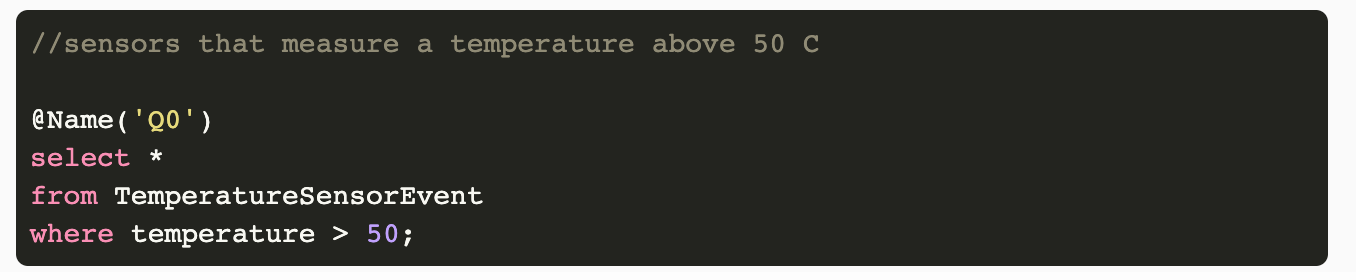
\includegraphics[width=400pt]{images/epl_Q0}\hspace*{\fill}
\end{figure}
\myparagraph{KSQL}
\begin{figure}[h!]
 \hfill 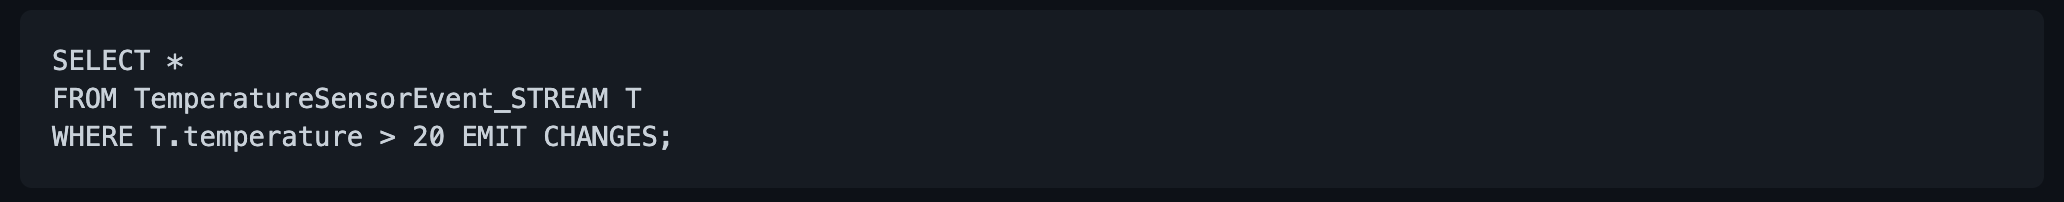
\includegraphics[width=400pt]{images/ksql_Q0}\hspace*{\fill}
\end{figure}
\myparagraph{Spark Structured Streaming}
\begin{figure}[h!]
 \hfill 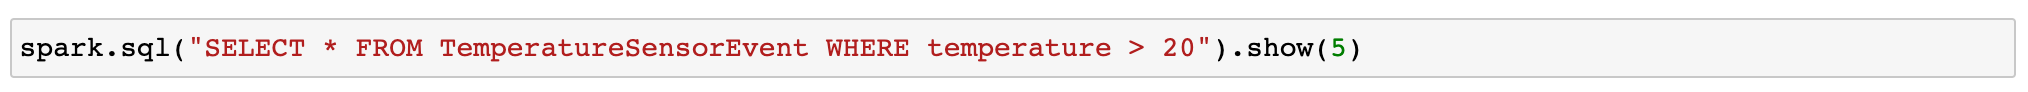
\includegraphics[width=400pt]{images/sss_Q0}\hspace*{\fill}
\end{figure}
\myparagraph{Flux}
\begin{figure}[h!]
 \hfill 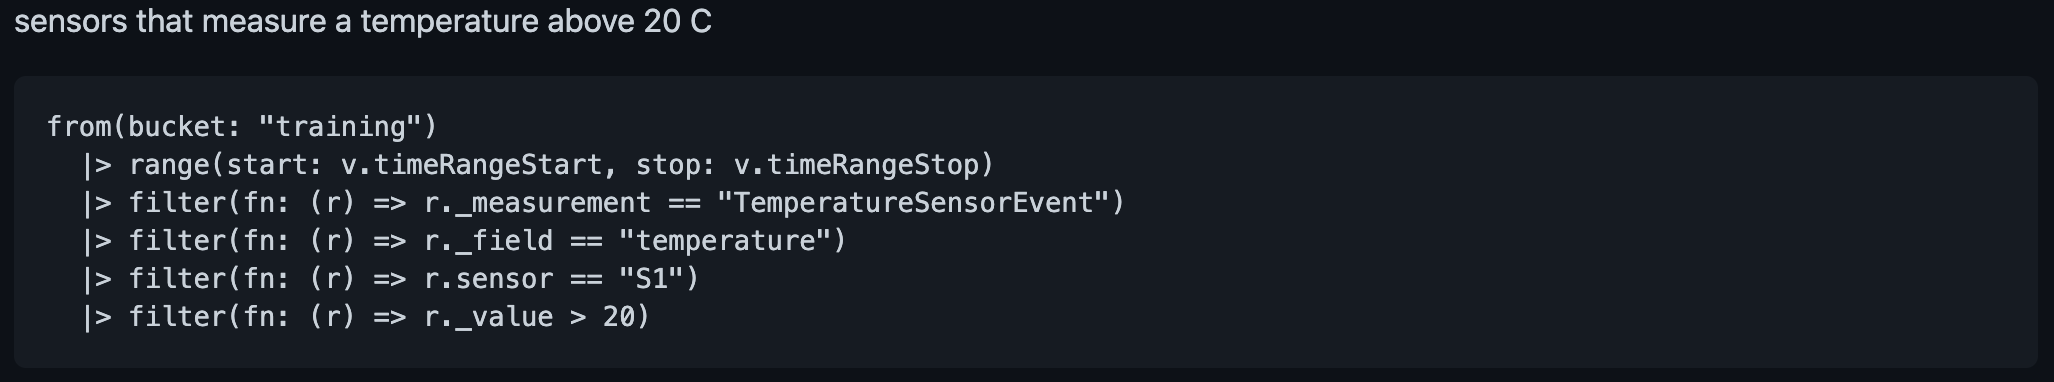
\includegraphics[width=400pt]{images/flux_Q0}\hspace*{\fill}
\end{figure}

\pagebreak

\subsection{Q1: sensors that observe smoke (smoke=true)}

\myparagraph{EPL}
\begin{figure}[h!]
 \hfill 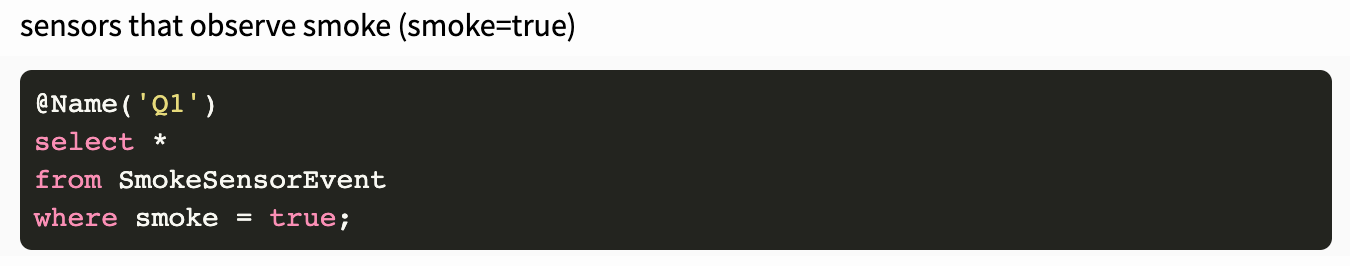
\includegraphics[width=400pt]{images/epl_Q1}\hspace*{\fill}
\end{figure}
\myparagraph{KSQL}
\begin{figure}[h!]
 \hfill 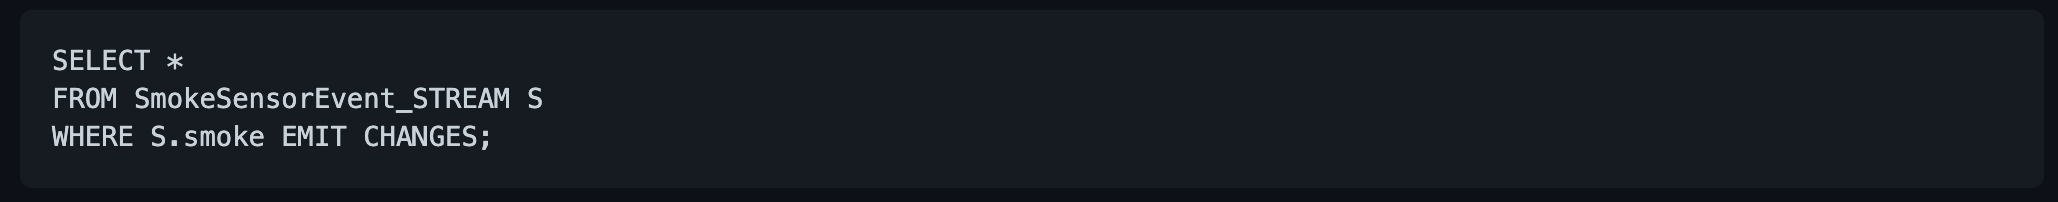
\includegraphics[width=400pt]{images/ksql_Q1}\hspace*{\fill}
\end{figure}
\myparagraph{Spark Structured Streaming}
\begin{figure}[h!]
 \hfill 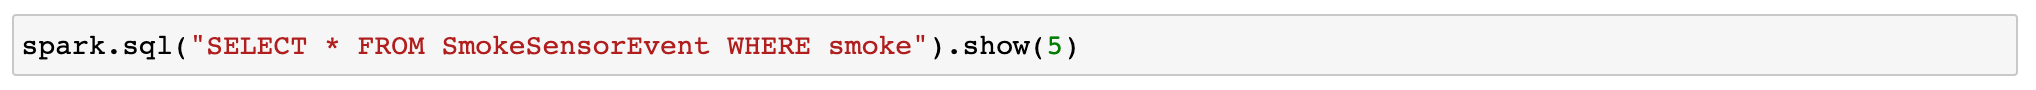
\includegraphics[width=400pt]{images/sss_Q1}\hspace*{\fill}
\end{figure}
\myparagraph{Flux}
\begin{figure}[h!]
 \hfill 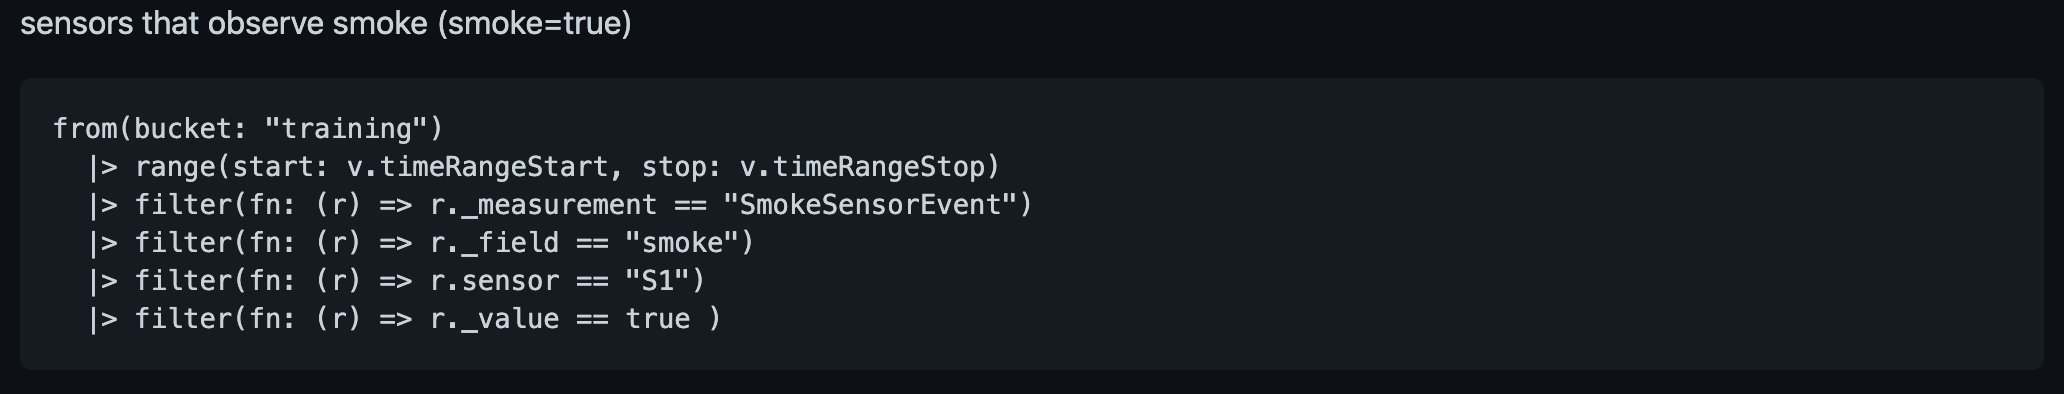
\includegraphics[width=400pt]{images/flux_Q1}\hspace*{\fill}
\end{figure}

\pagebreak

\subsection{Q2: the average temperature observed by the sensors}

\myparagraph{EPL}
\begin{figure}[h!]
 \hfill 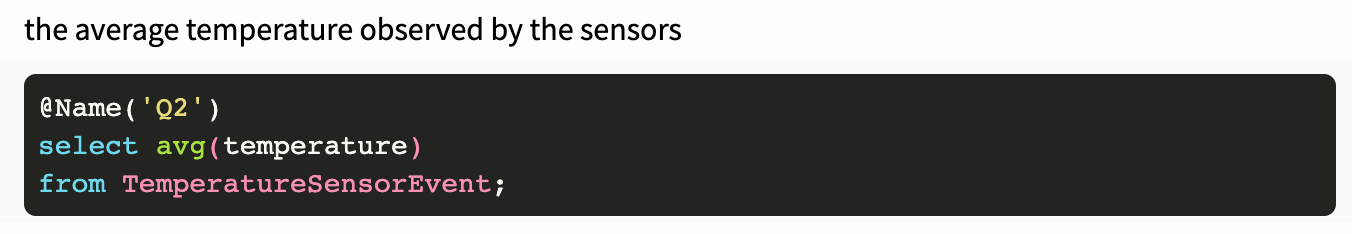
\includegraphics[width=400pt]{images/epl_Q2}\hspace*{\fill}
\end{figure}
\myparagraph{KSQL}
\begin{figure}[h!]
 \hfill 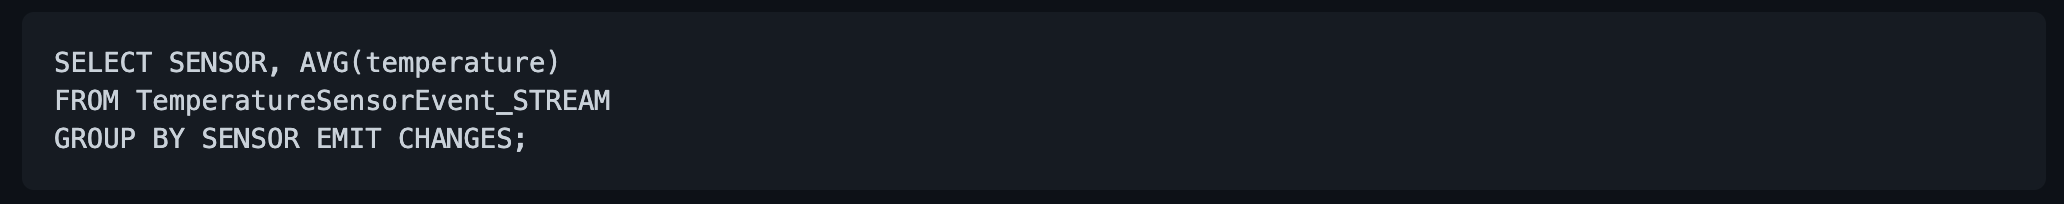
\includegraphics[width=400pt]{images/ksql_Q2}\hspace*{\fill}
\end{figure}
\myparagraph{Spark Structured Streaming}
\begin{figure}[h!]
 \hfill 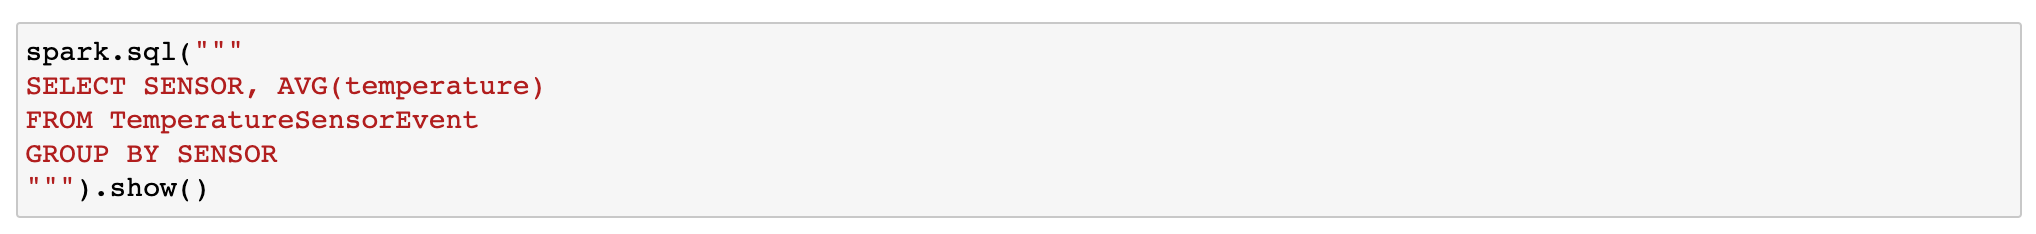
\includegraphics[width=400pt]{images/sss_Q2}\hspace*{\fill}
\end{figure}
\myparagraph{Flux}
\begin{figure}[h!]
 \hfill 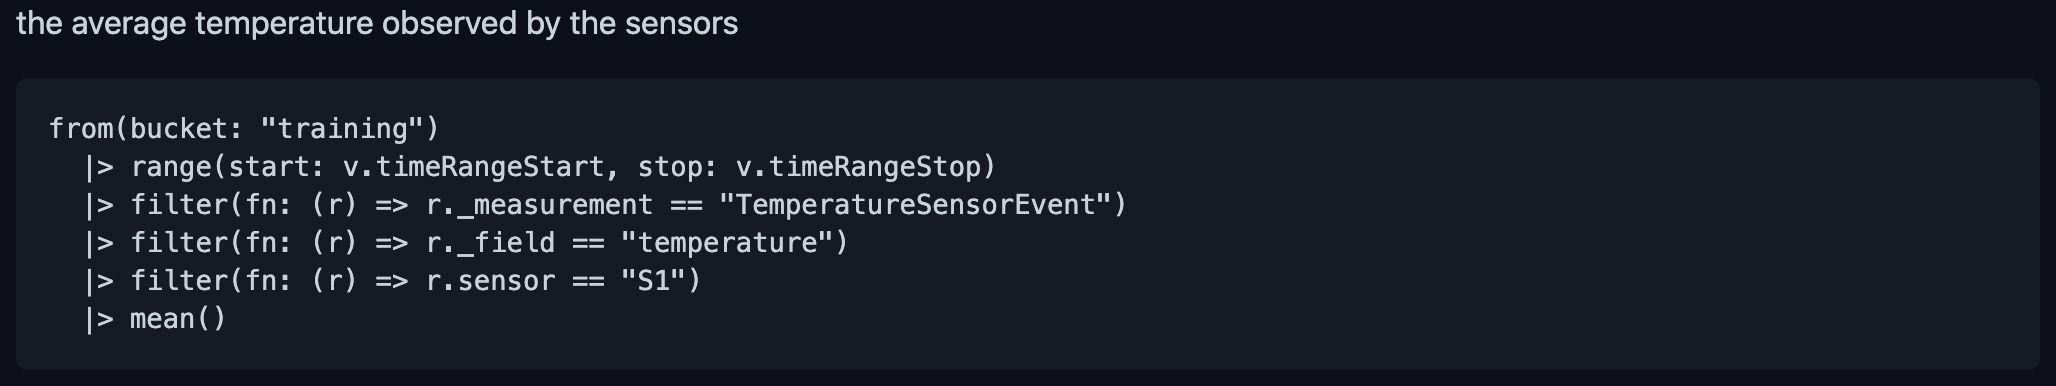
\includegraphics[width=400pt]{images/flux_Q2}\hspace*{\fill}
\end{figure}

\pagebreak

\subsection{Q3 (logical sliding window): the average temperature observed by the sensors in the last 4 seconds}

\myparagraph{EPL}
\begin{figure}[h!]
 \hfill 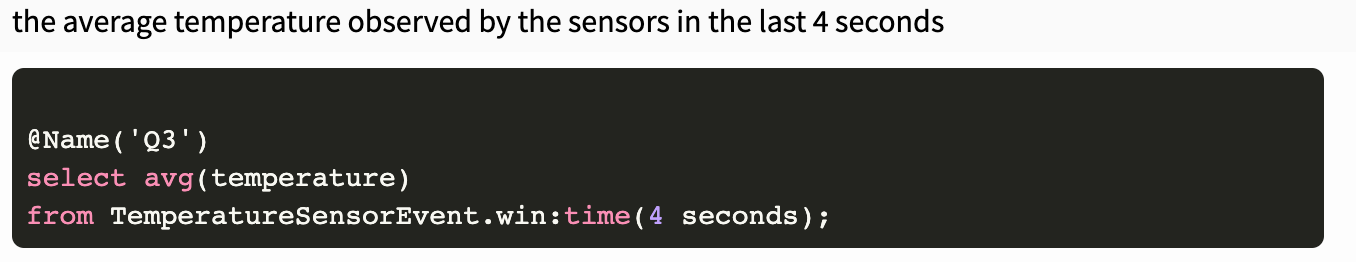
\includegraphics[width=400pt]{images/epl_Q3}\hspace*{\fill}
\end{figure}
\myparagraph{KSQL}
Not supported
\myparagraph{Spark Structured Streaming}
Not supported
\myparagraph{Flux}
\begin{figure}[h!]
 \hfill 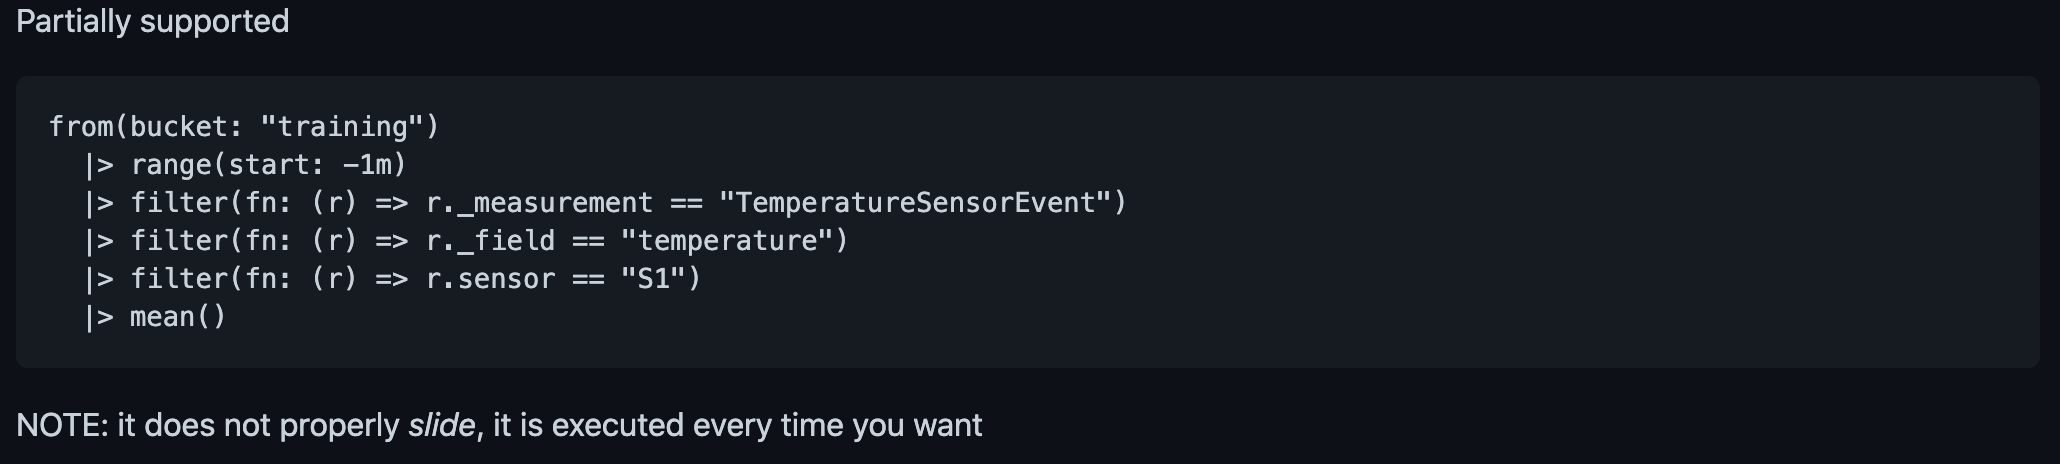
\includegraphics[width=400pt]{images/flux_Q3}\hspace*{\fill}
\end{figure}

\pagebreak

\subsection{Q4 (logical tumbling window): the average temperature observed by the sensors in the last 4 seconds updating the window after 4 seconds}

\myparagraph{EPL}
\begin{figure}[h!]
 \hfill 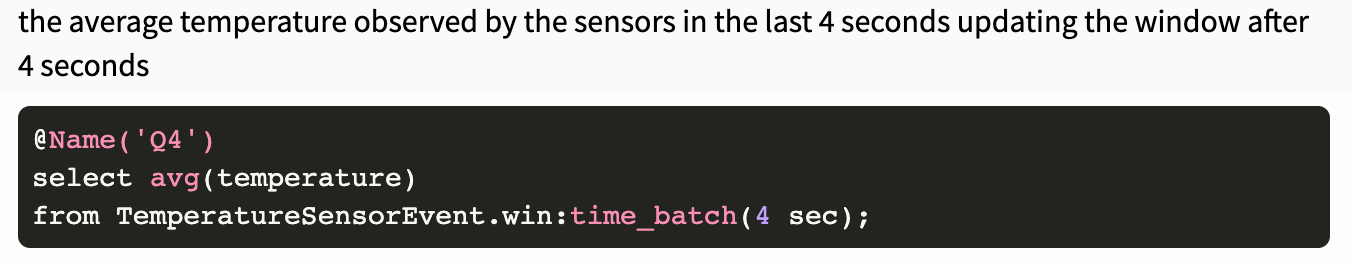
\includegraphics[width=400pt]{images/epl_Q4}\hspace*{\fill}
\end{figure}
\myparagraph{KSQL}
\begin{figure}[h!]
 \hfill 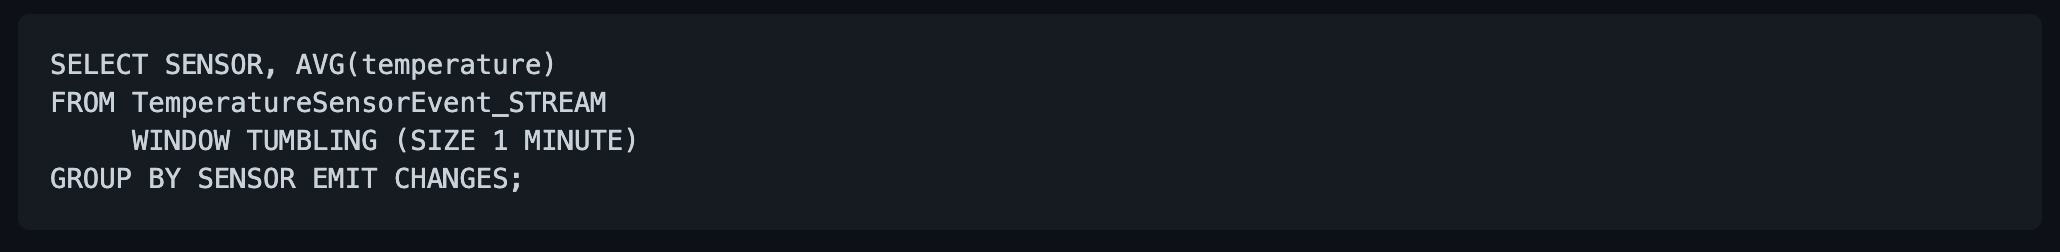
\includegraphics[width=400pt]{images/ksql_Q4}\hspace*{\fill}
\end{figure}
\myparagraph{Spark Structured Streaming}
\begin{figure}[h!]
 \hfill 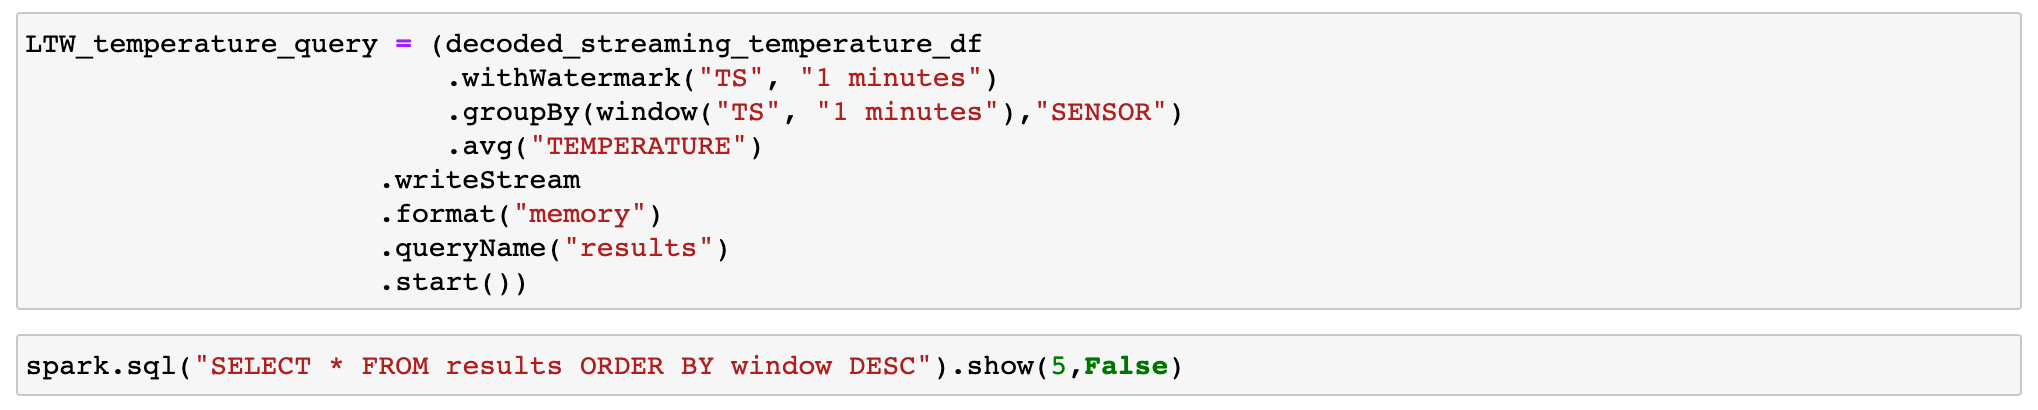
\includegraphics[width=400pt]{images/sss_Q4}\hspace*{\fill}
\end{figure}
\myparagraph{Flux}
\begin{figure}[h!]
 \hfill 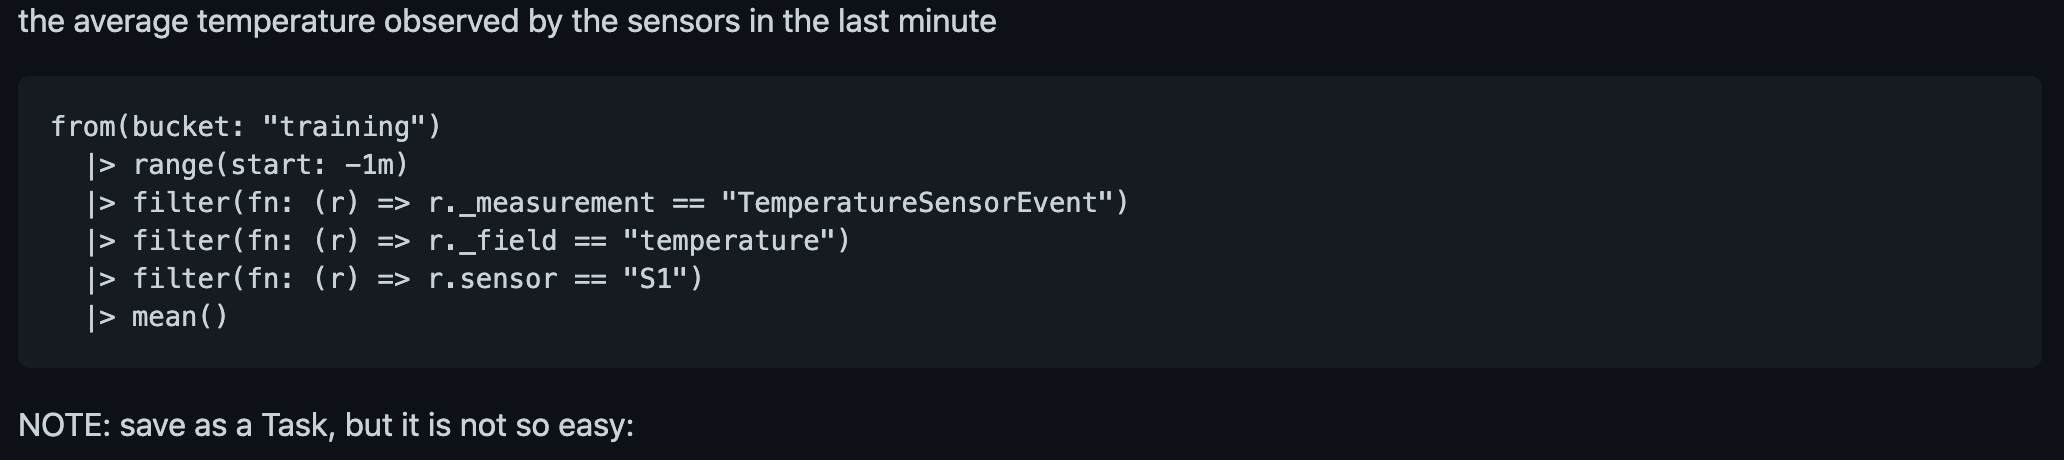
\includegraphics[width=400pt]{images/flux_Q4}\hspace*{\fill}
\end{figure} \\
Saves as a task and execute it every minute

\pagebreak

\subsection{Q5 (phyisical sliding window): the average temperature observed by the sensors in the last 5 events}

\myparagraph{EPL}
\begin{figure}[h!]
 \hfill 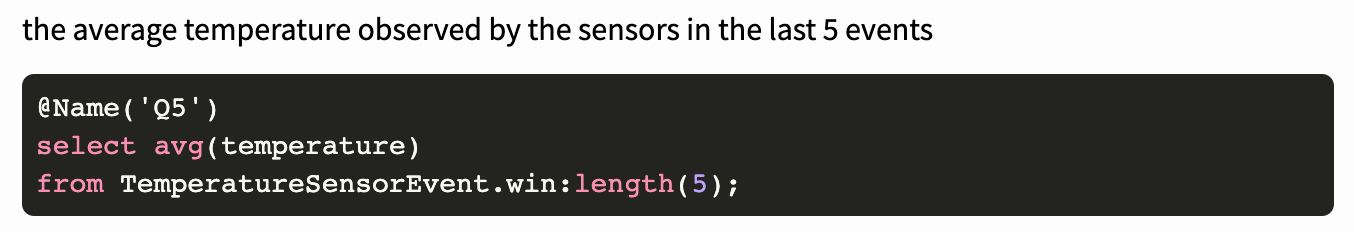
\includegraphics[width=400pt]{images/epl_Q5}\hspace*{\fill}
\end{figure}
\myparagraph{KSQL}
Not supported
\myparagraph{Spark Structured Streaming}
Not supported
\myparagraph{Flux}
\begin{figure}[h!]
 \hfill 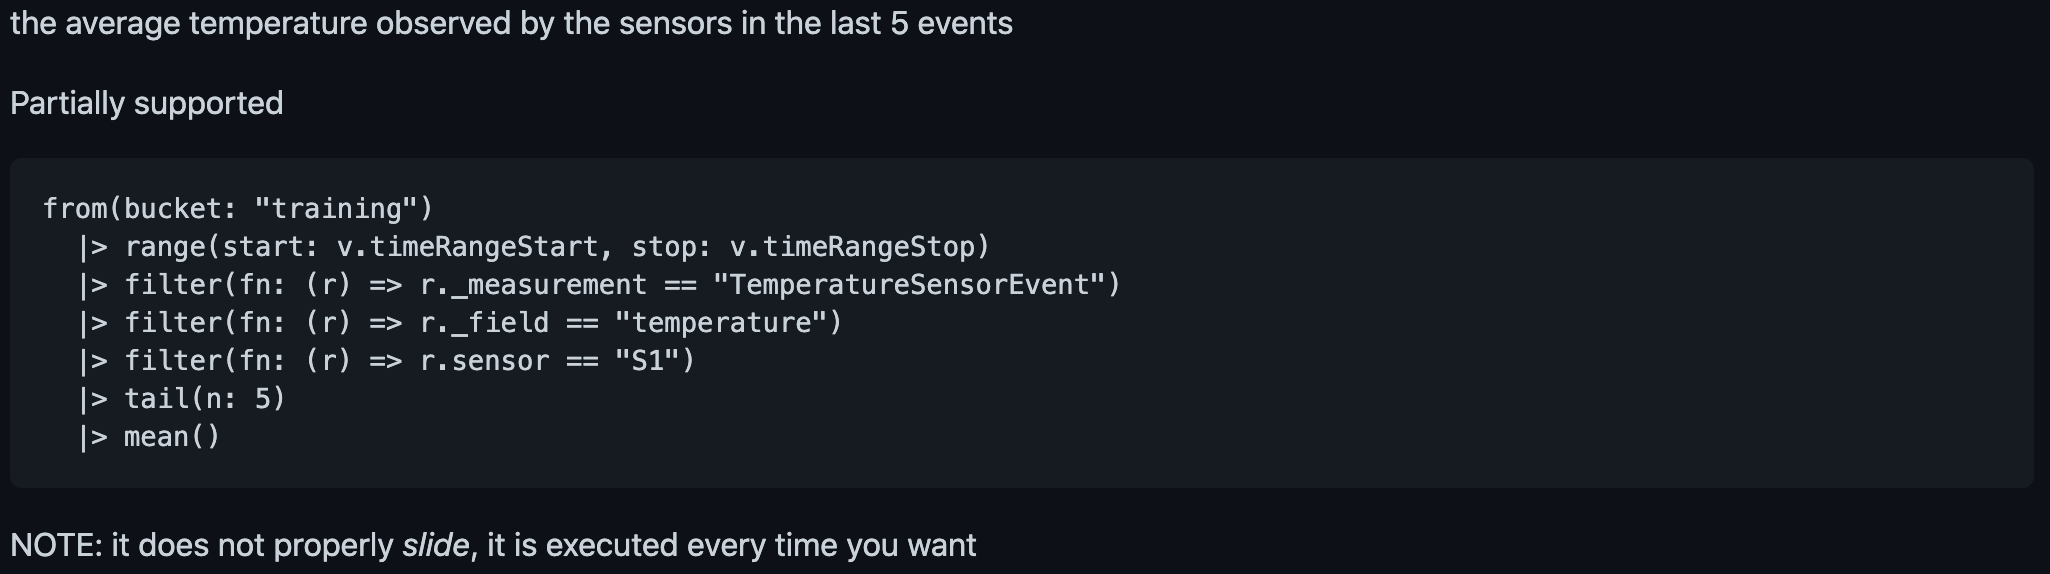
\includegraphics[width=400pt]{images/flux_Q5}\hspace*{\fill}
\end{figure}

\pagebreak

\subsection{Q6 (phyisical tumbling window): the average temperature observed by the sensors in the last 5 events updating the window after 5 events}

\myparagraph{EPL}
\begin{figure}[h!]
 \hfill 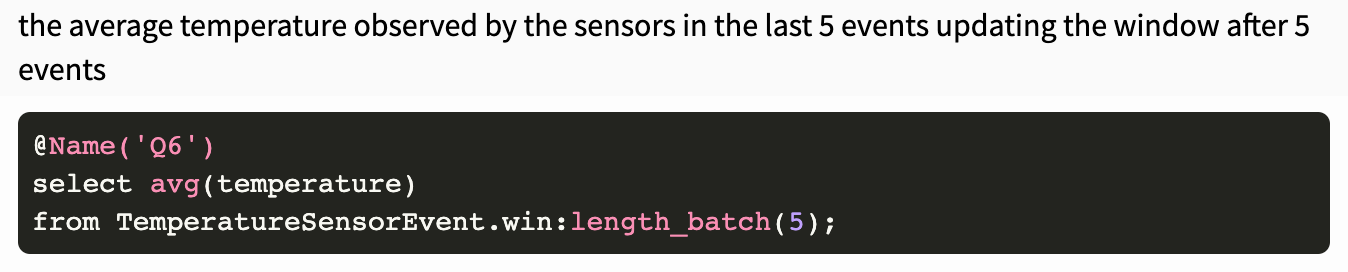
\includegraphics[width=400pt]{images/epl_Q6}\hspace*{\fill}
\end{figure}
\myparagraph{KSQL}
Not supported
\myparagraph{Spark Structured Streaming}
Not supported
\myparagraph{Flux}
\begin{figure}[h!]
 \hfill 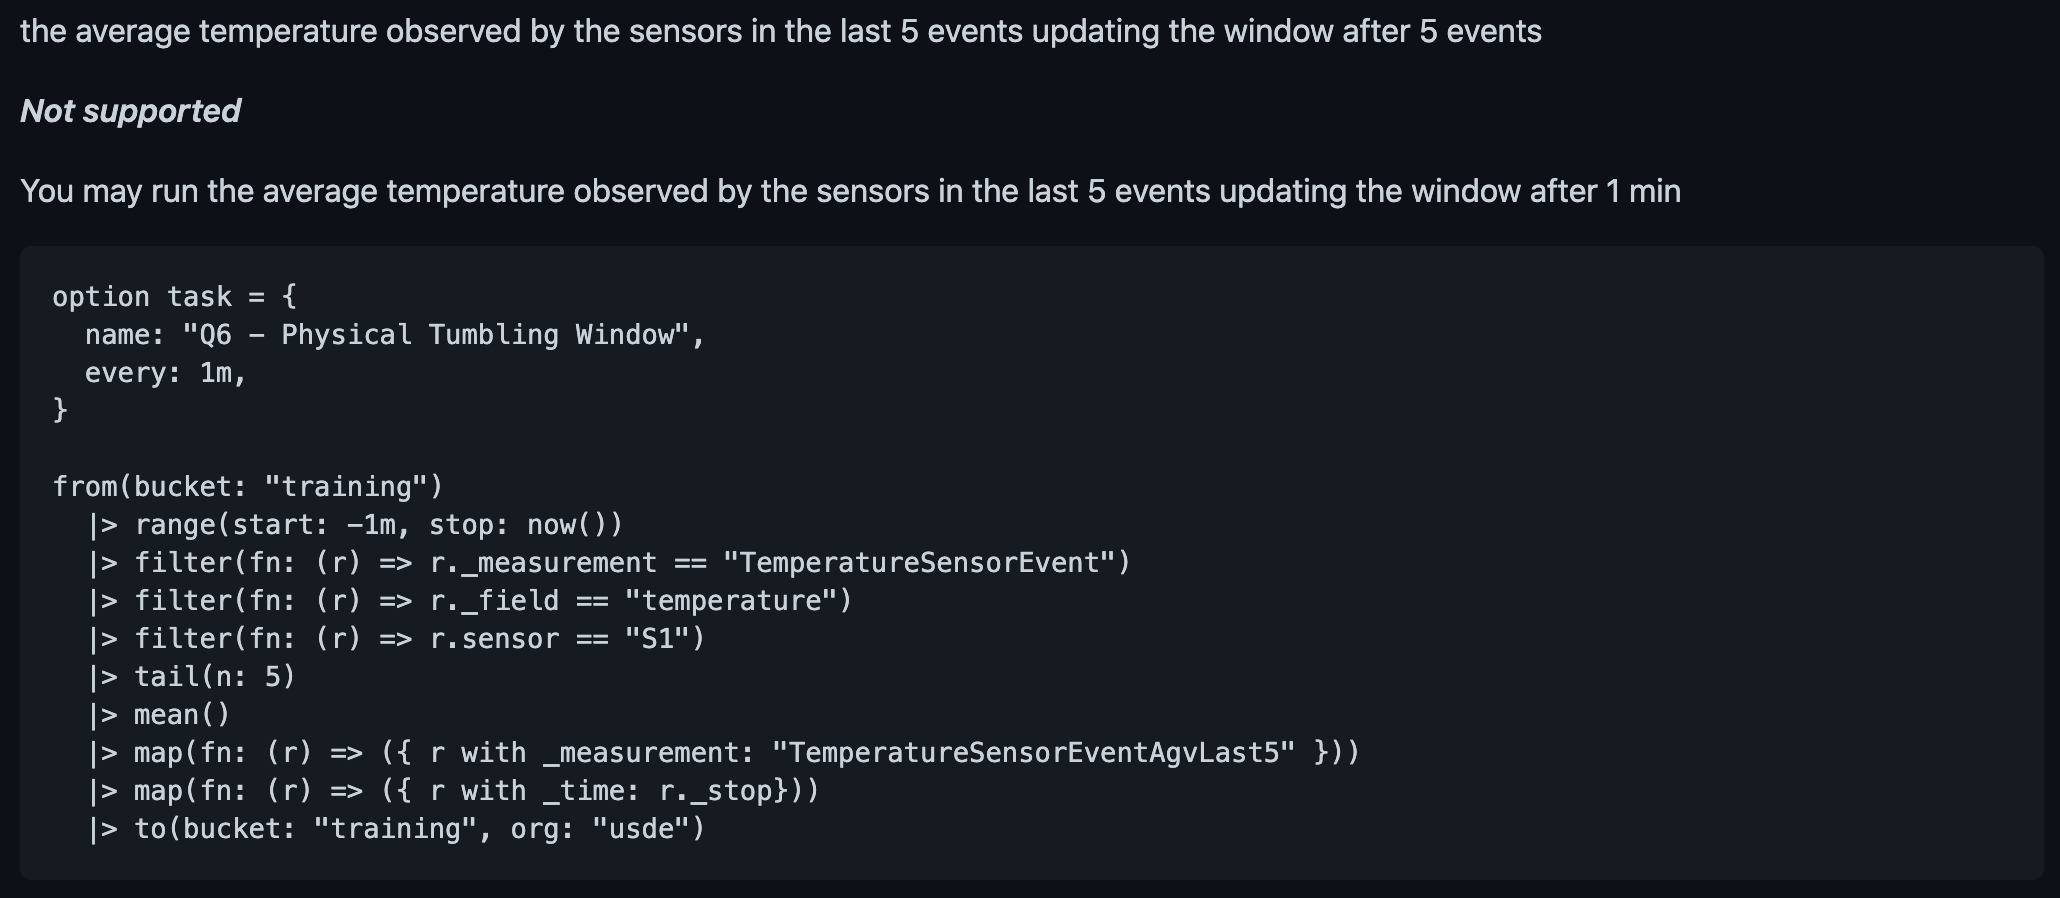
\includegraphics[width=400pt]{images/flux_Q6}\hspace*{\fill}
\end{figure}

\pagebreak

\subsection{Q7 (logical hopping window): the average temperature observed by the sensors in the last 4 seconds computed every 2 seconds}

\myparagraph{EPL}
\begin{figure}[h!]
 \hfill 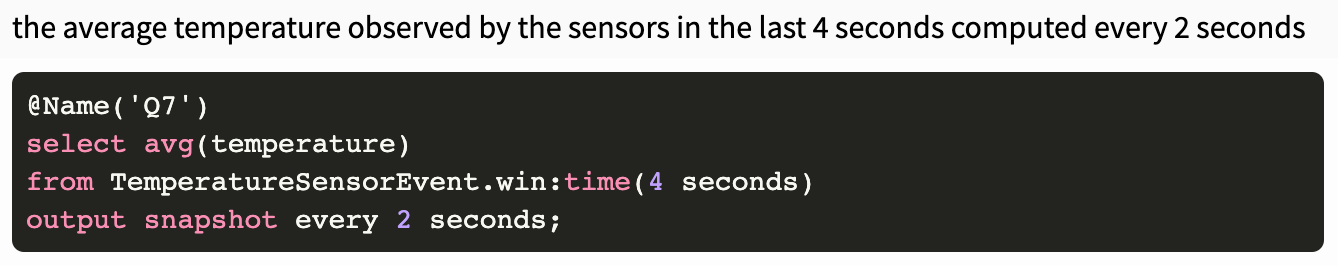
\includegraphics[width=400pt]{images/epl_Q7}\hspace*{\fill}
\end{figure}
\myparagraph{KSQL}
\begin{figure}[h!]
 \hfill 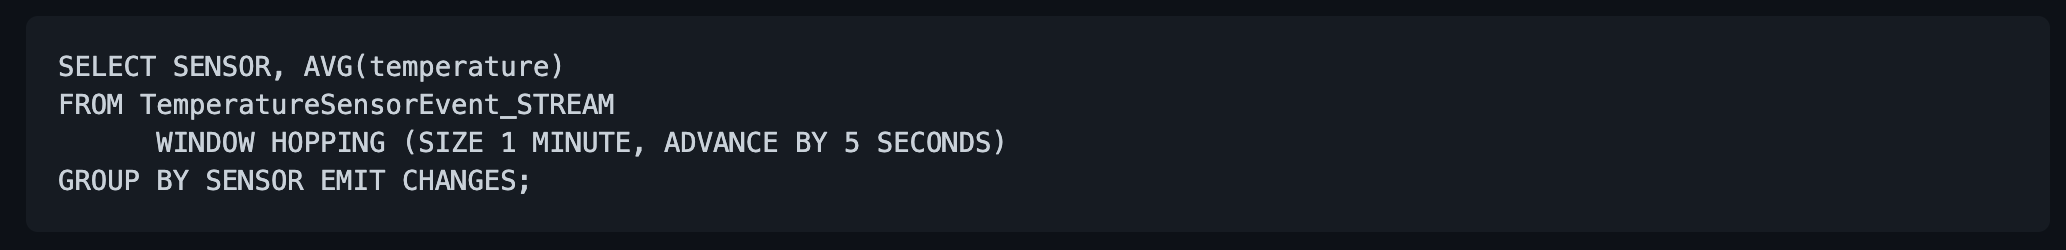
\includegraphics[width=400pt]{images/ksql_Q7}\hspace*{\fill}
\end{figure}
\myparagraph{Spark Structured Streaming}
\begin{figure}[h!]
 \hfill 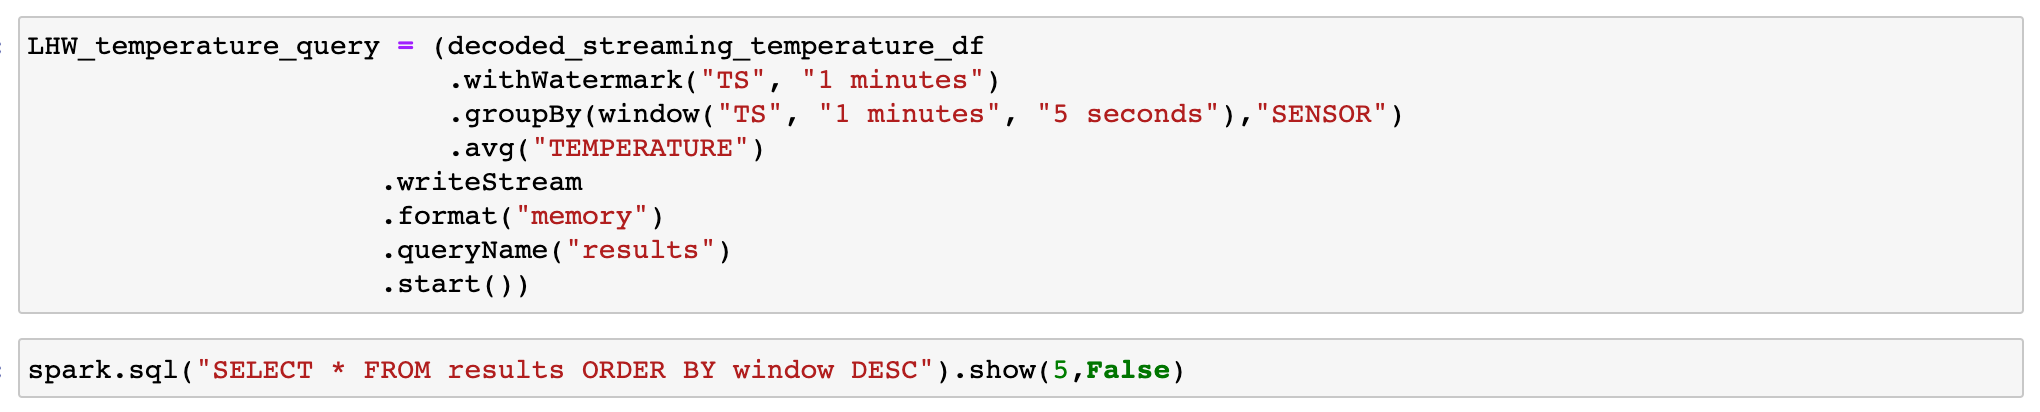
\includegraphics[width=400pt]{images/sss_Q7}\hspace*{\fill}
\end{figure}
\myparagraph{Flux}
\begin{figure}[h!]
 \hfill 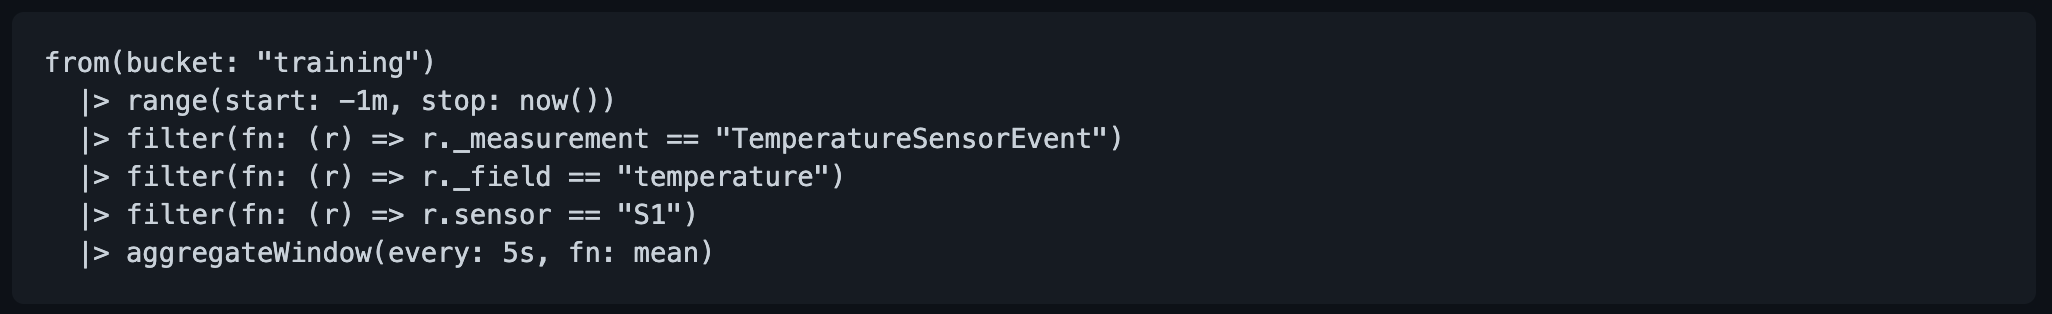
\includegraphics[width=400pt]{images/flux_Q7}\hspace*{\fill}
\end{figure}

\pagebreak

\subsection{Q8 \& Q9: stream-to-stream join and Fire Event detection}

\myparagraph{EPL}
\begin{figure}[h!]
 \hfill 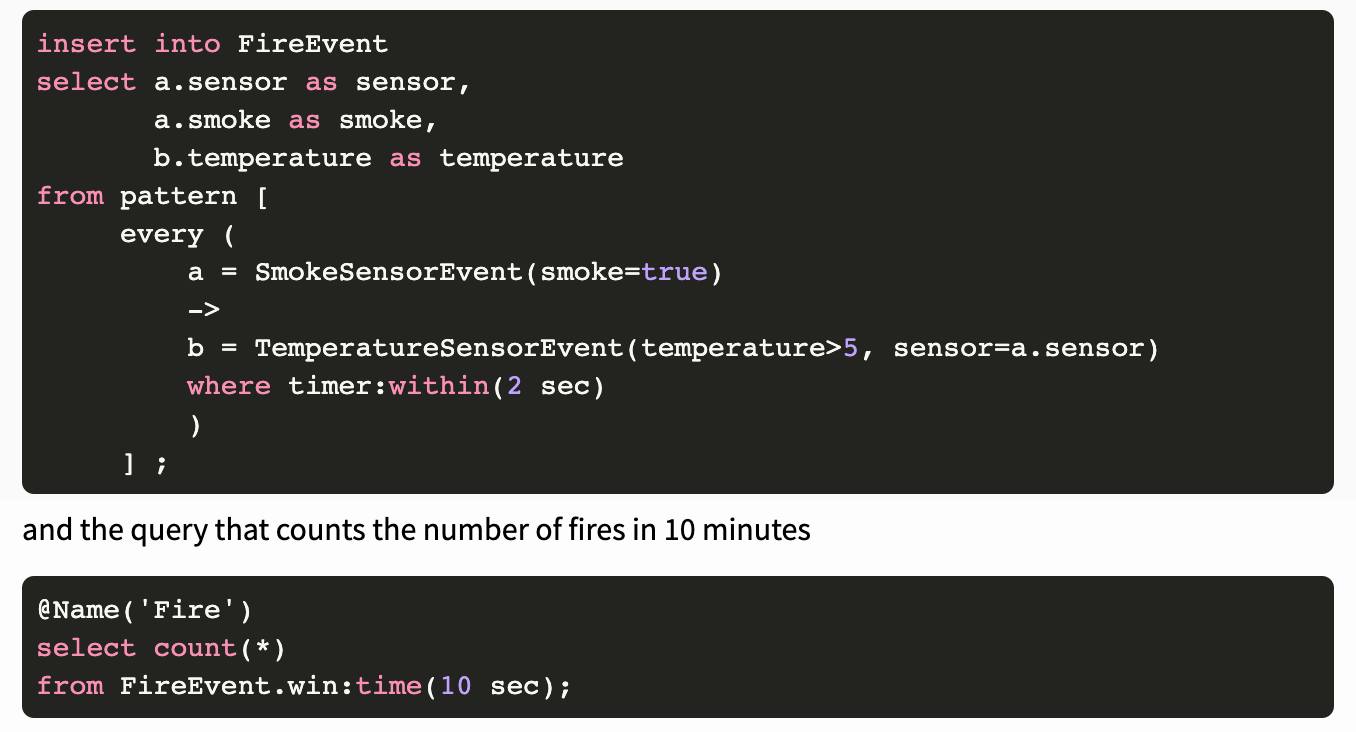
\includegraphics[width=400pt]{images/epl_Q8}\hspace*{\fill}
\end{figure}
\myparagraph{KSQL}
\begin{figure}[h!]
 \hfill 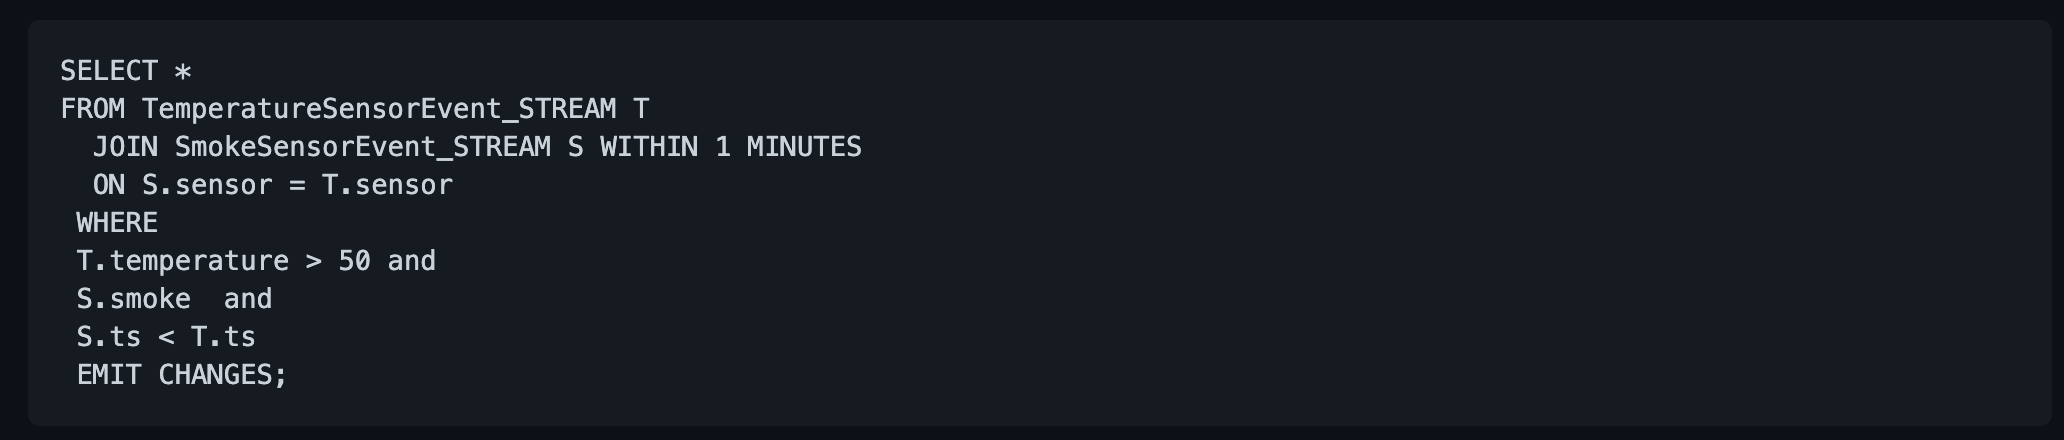
\includegraphics[width=400pt]{images/ksql_Q8}\hspace*{\fill}
 \\ \center
 \hfill 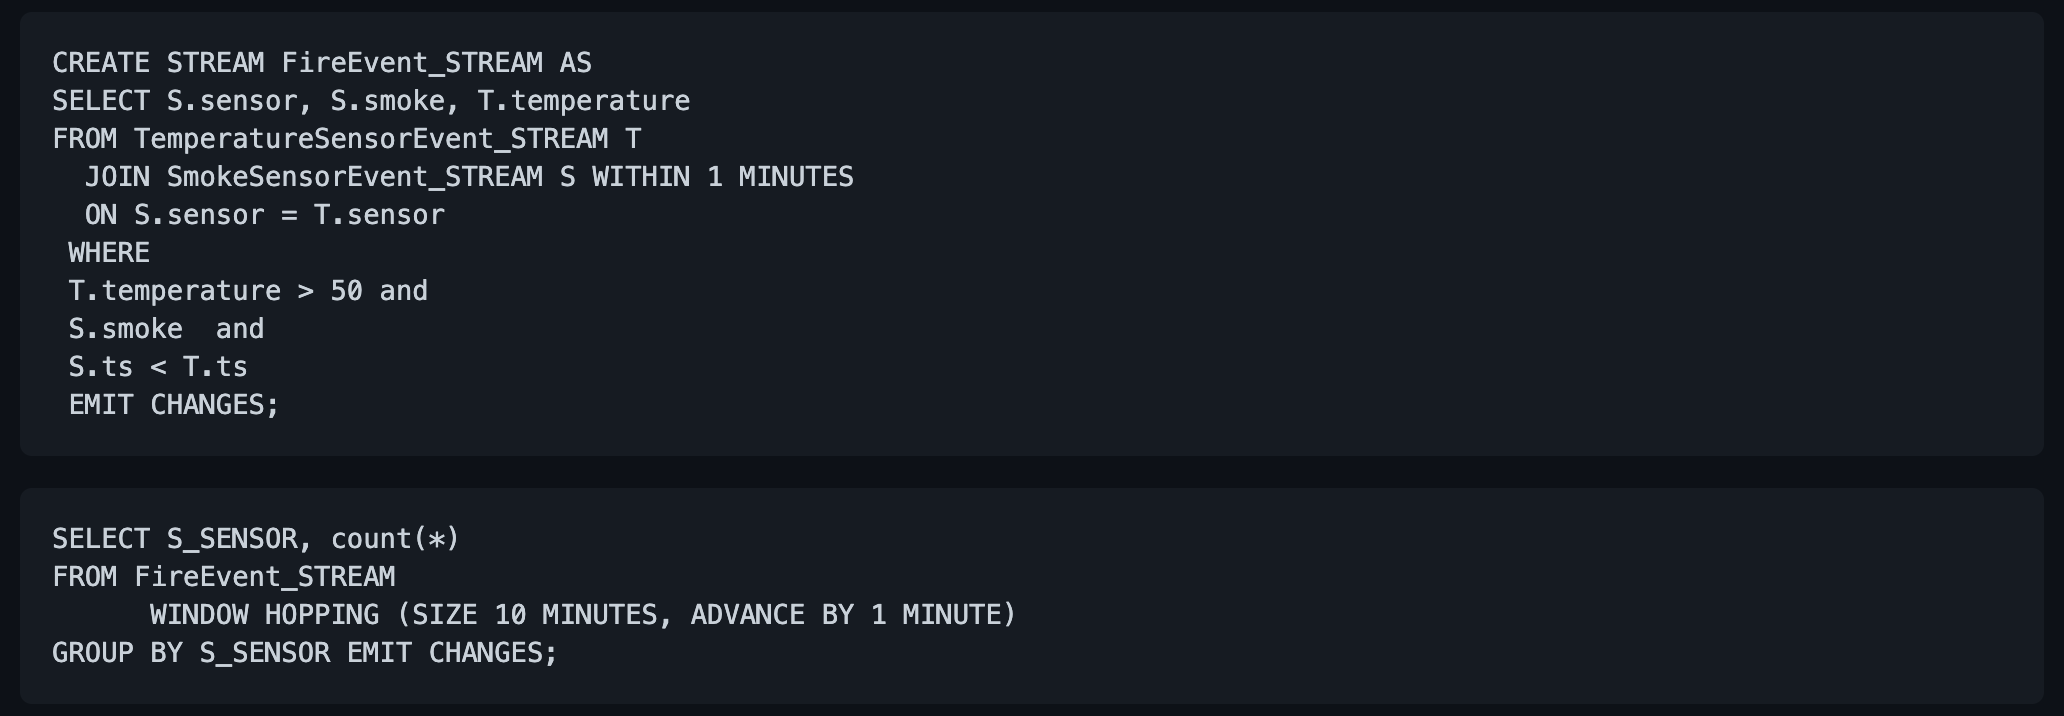
\includegraphics[width=400pt]{images/ksql_Q9}\hspace*{\fill}
\end{figure}
\pagebreak
\myparagraph{Spark Structured Streaming}
\begin{figure}[h!]
 \hfill 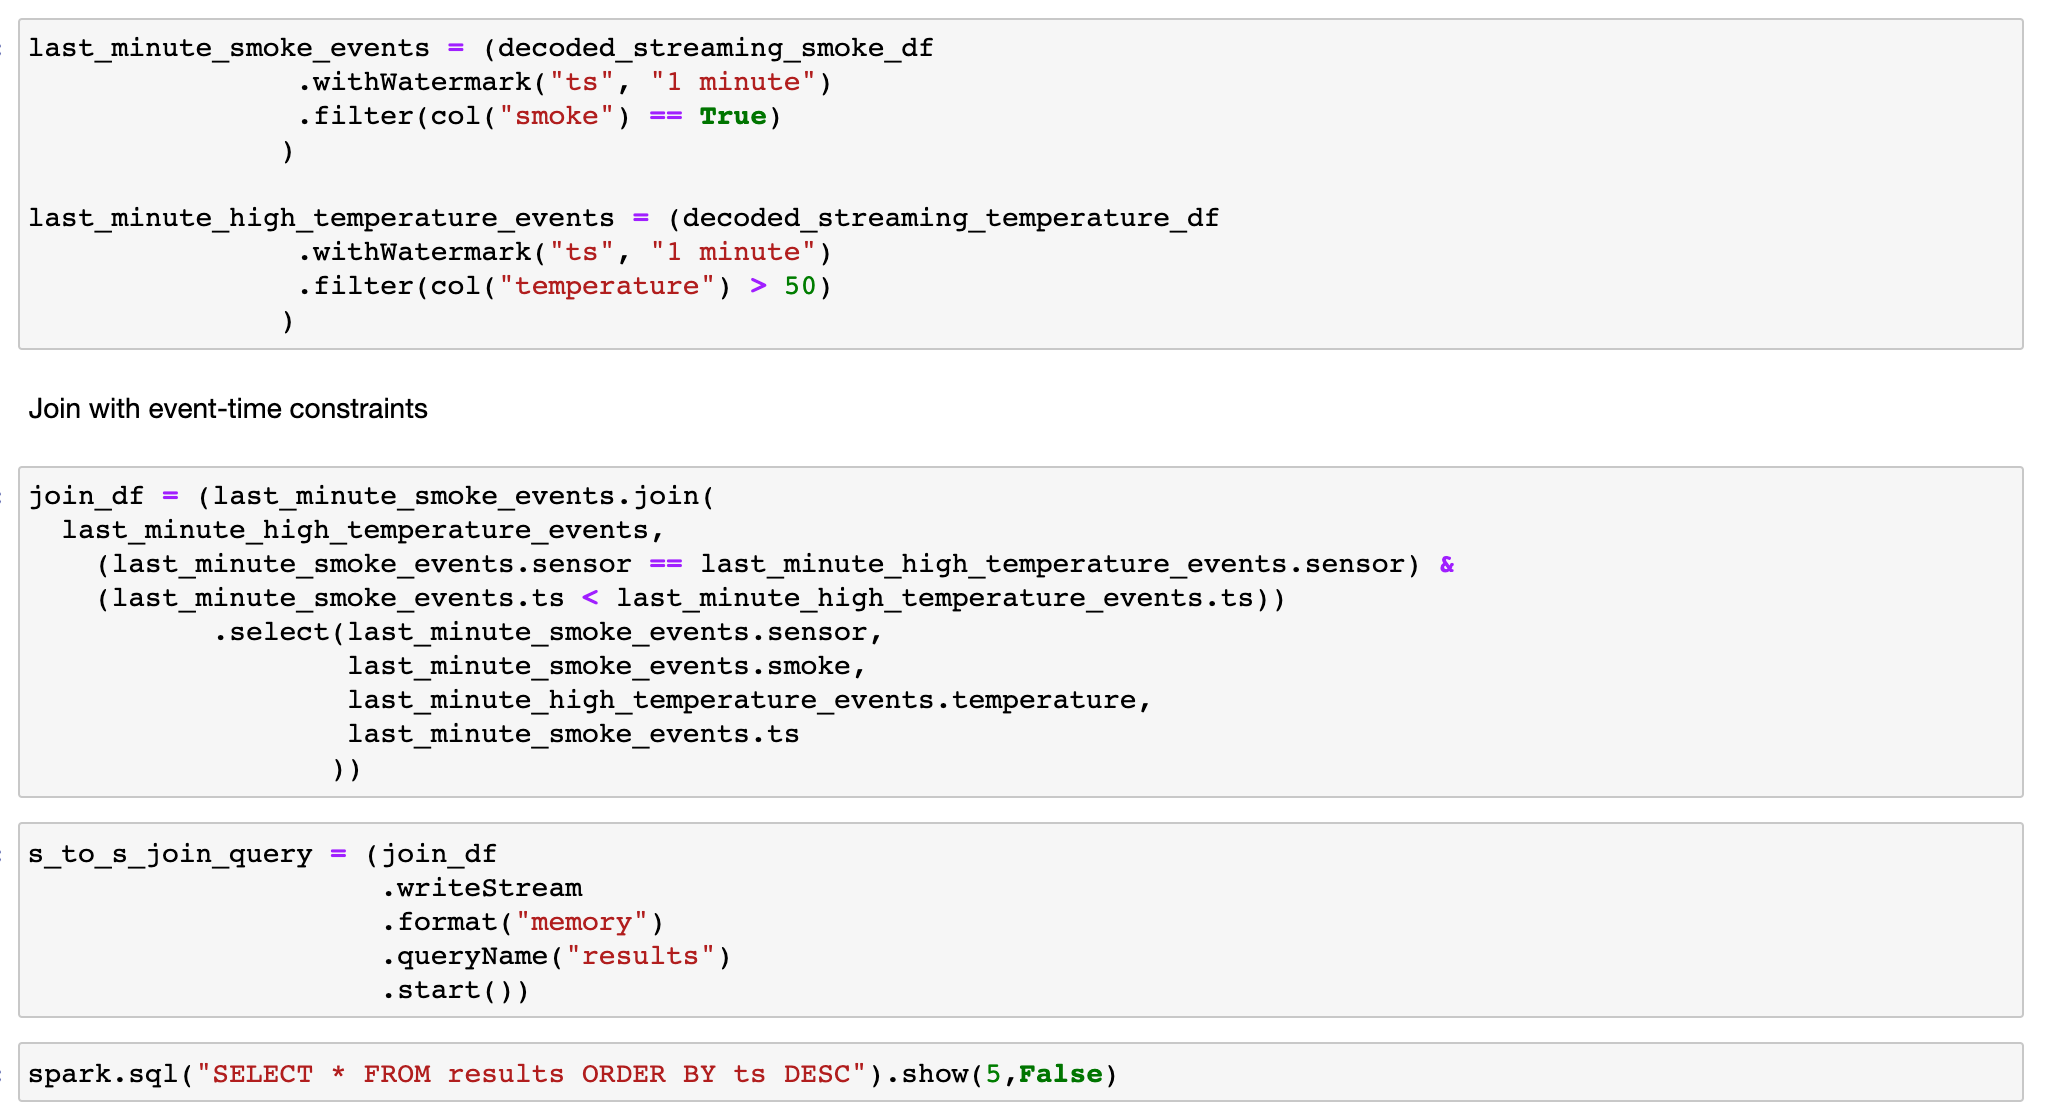
\includegraphics[width=400pt]{images/sss_Q8}\hspace*{\fill}
  \\ \center
   \hfill 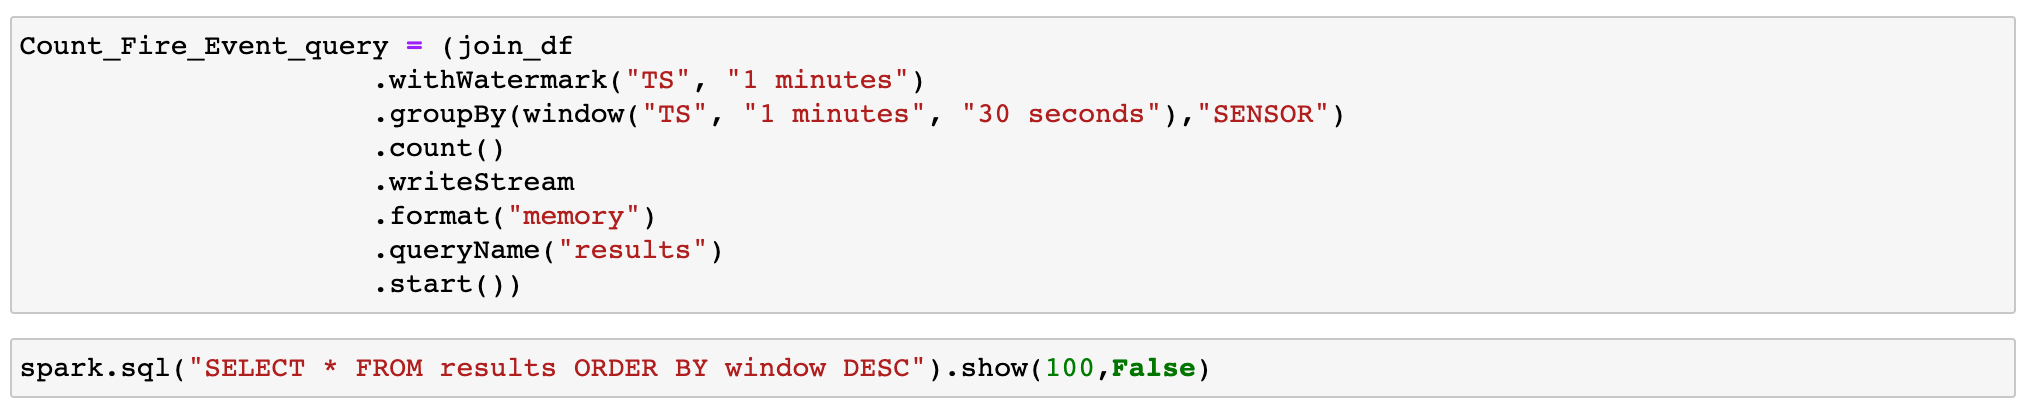
\includegraphics[width=400pt]{images/sss_Q9}\hspace*{\fill}
\end{figure}
\pagebreak
\myparagraph{Flux}
\begin{figure}[h!]
 \hfill 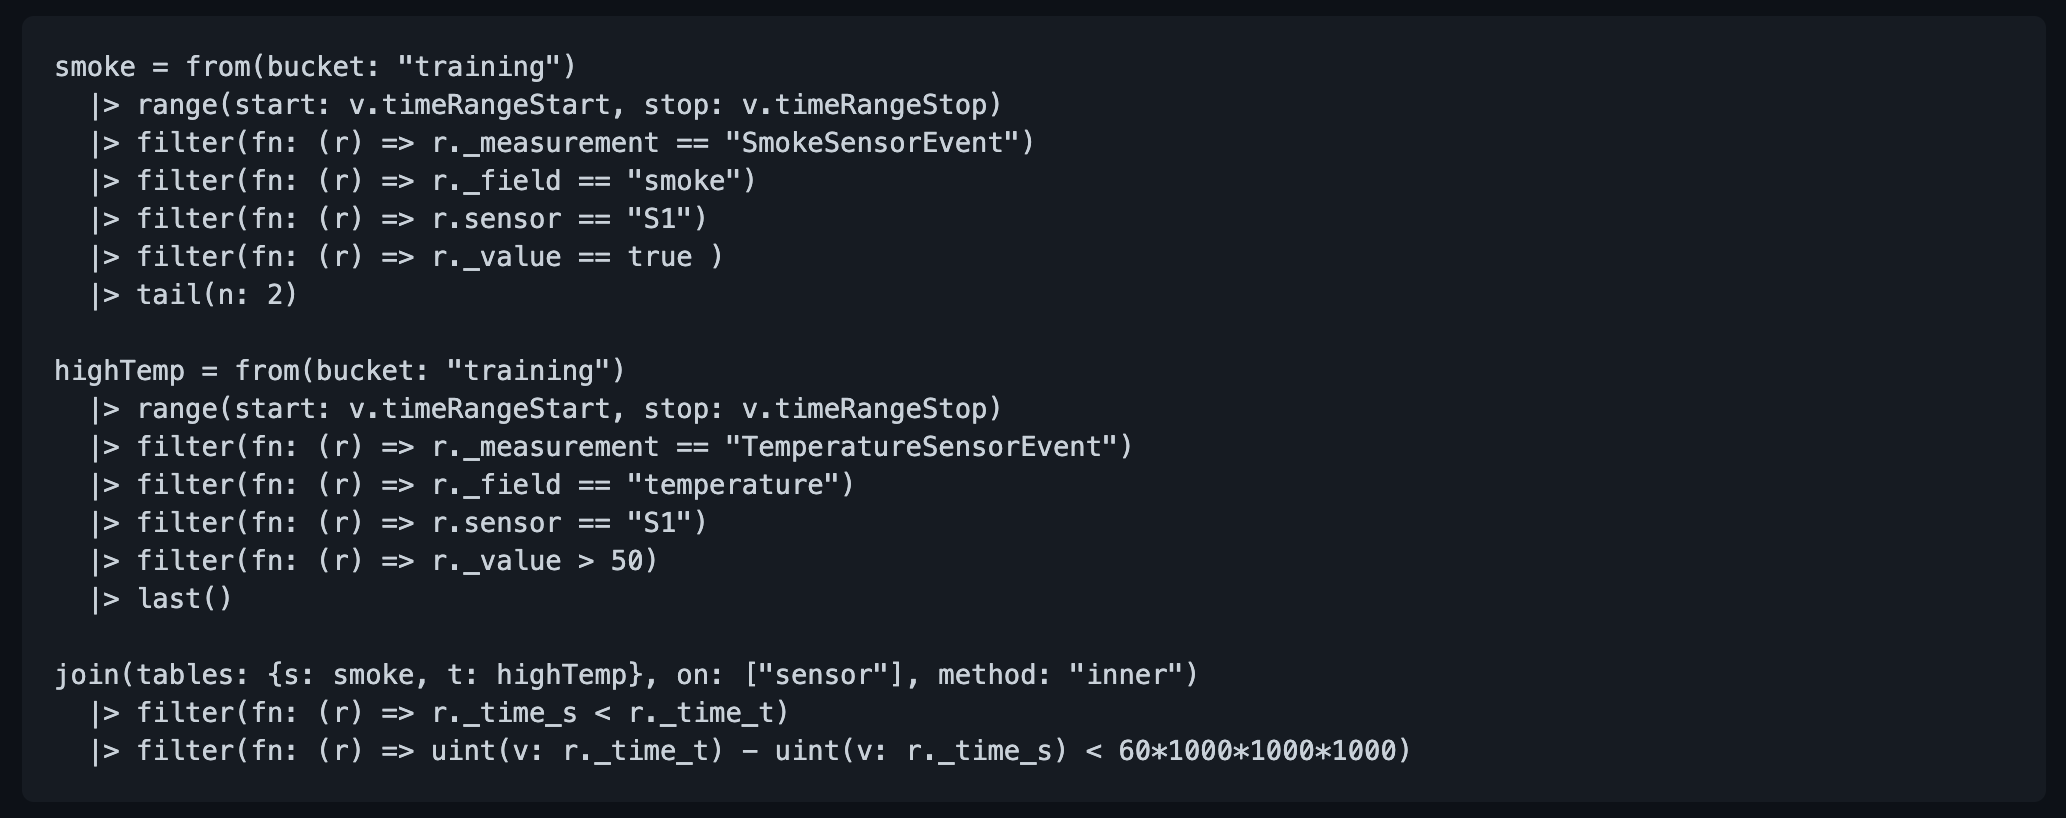
\includegraphics[width=400pt]{images/flux_Q8}\hspace*{\fill}
 \\ \center
  \hfill 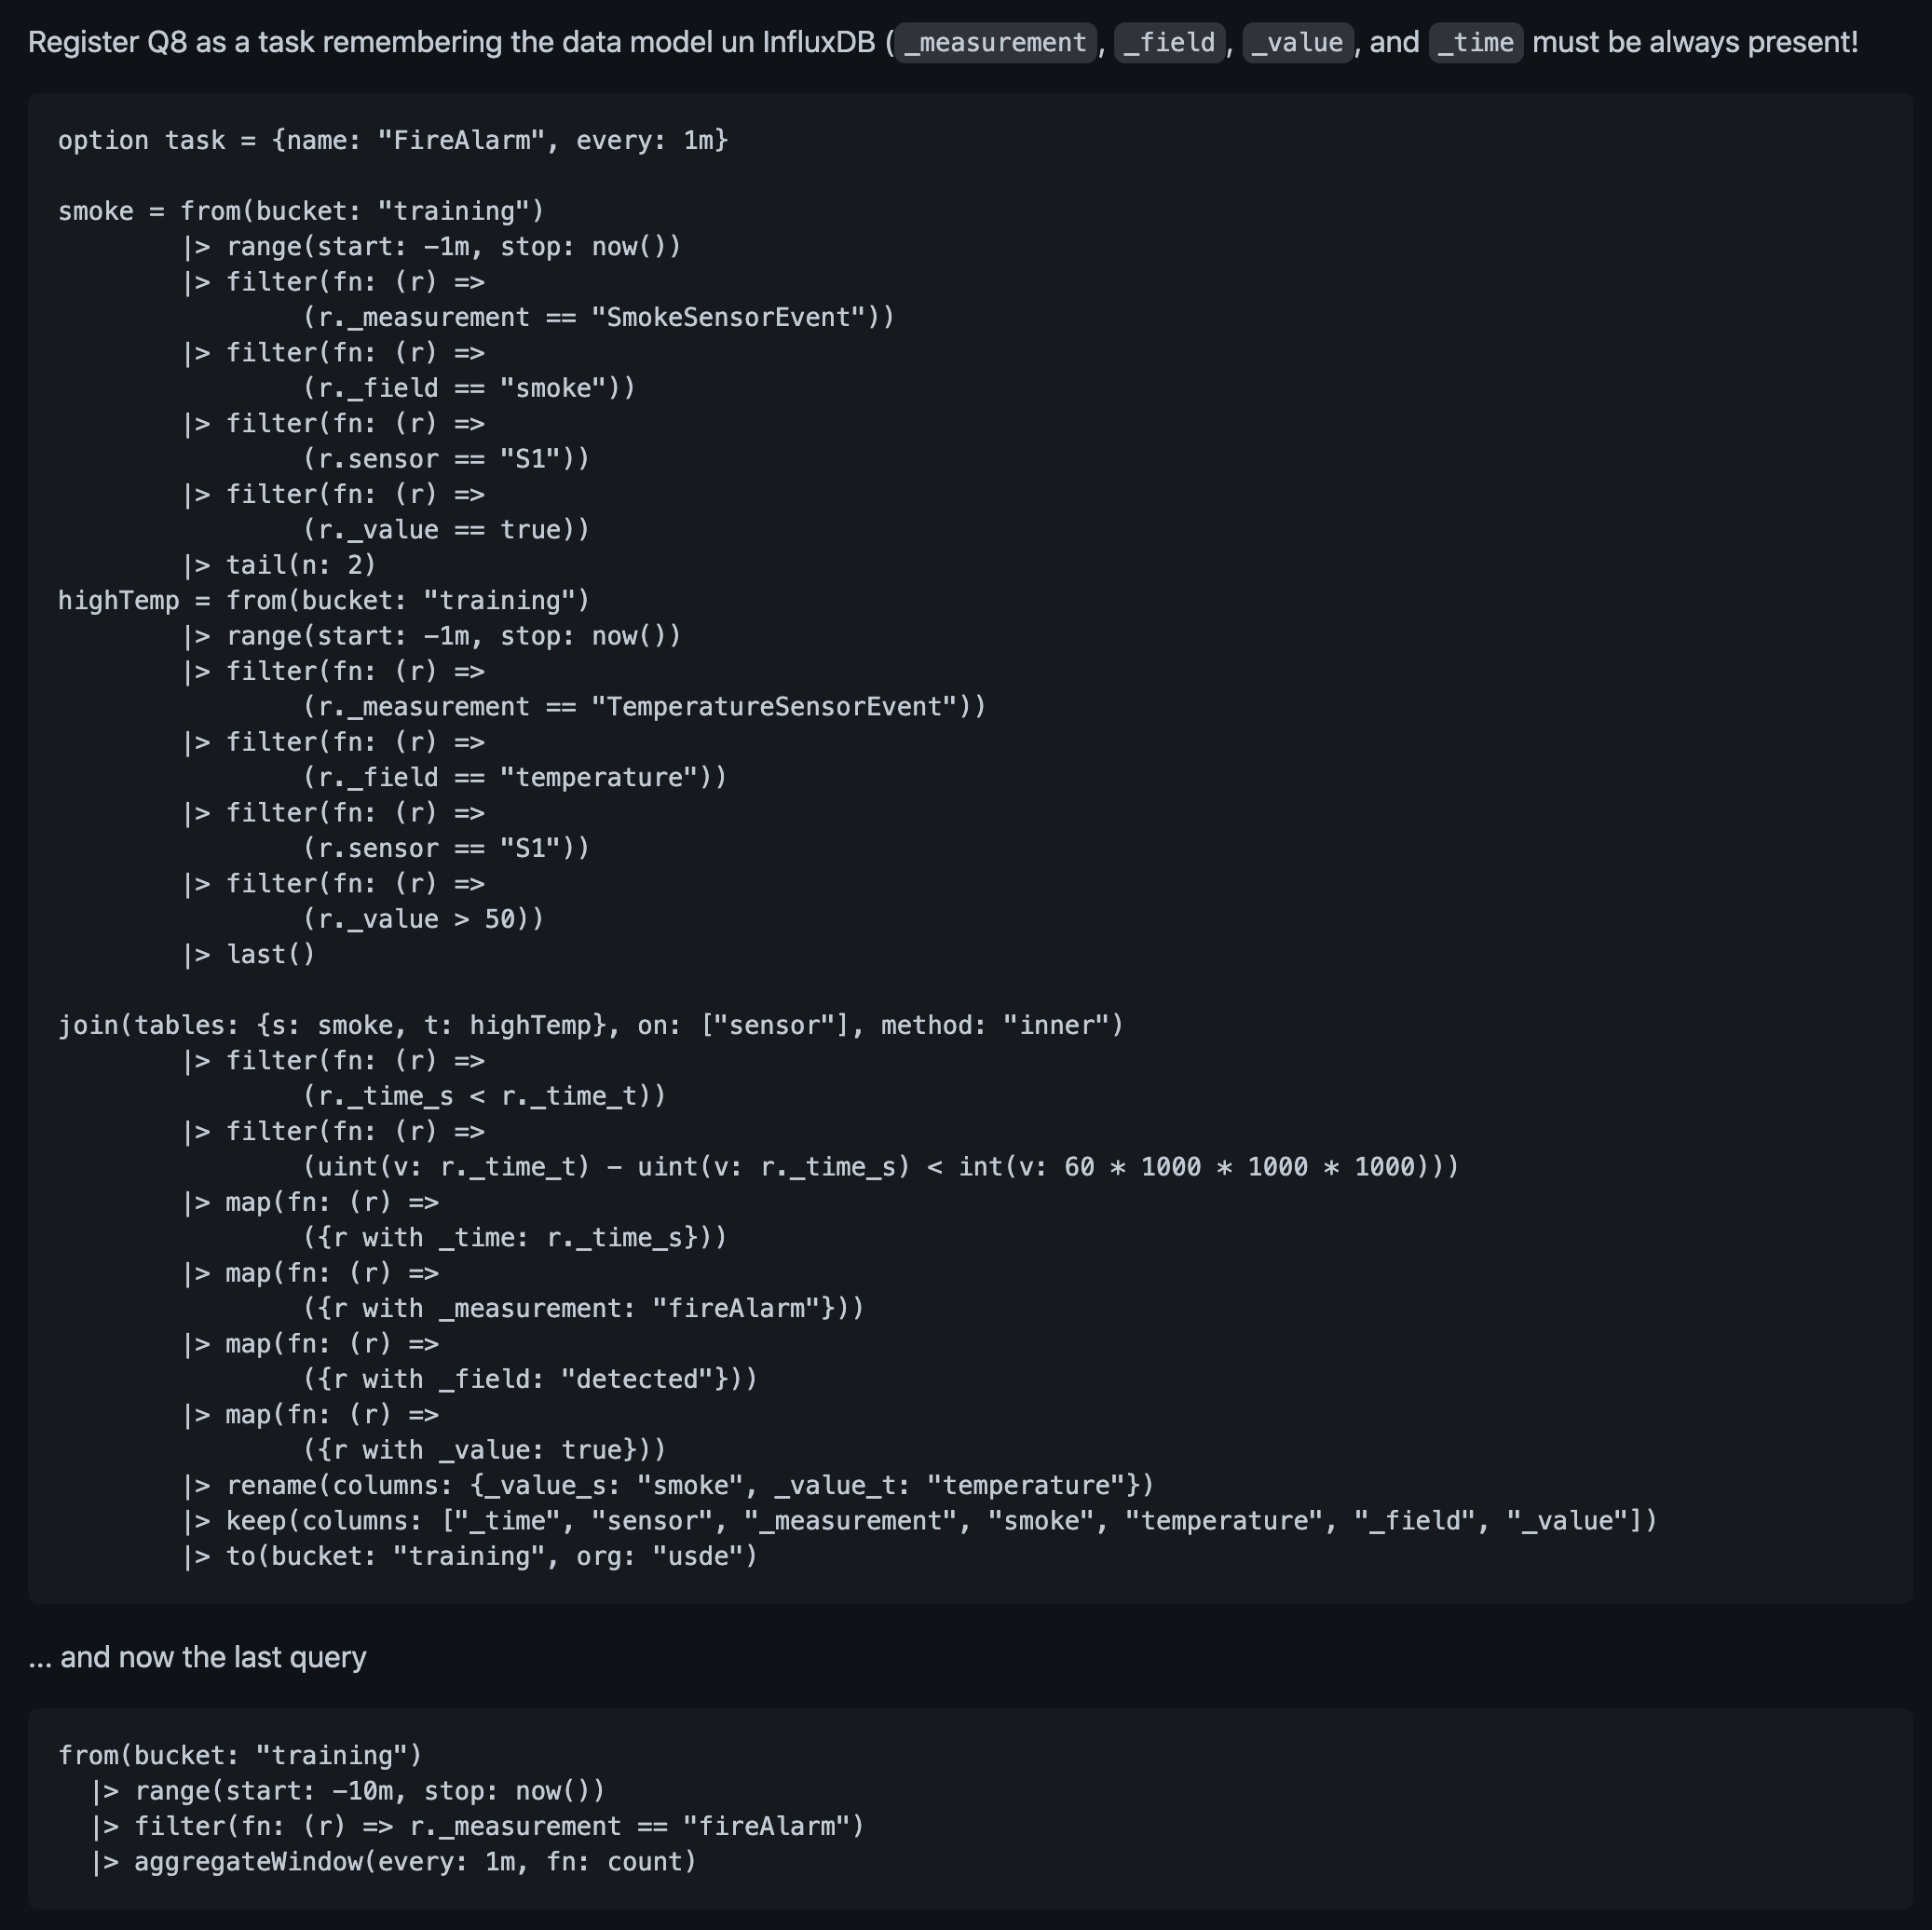
\includegraphics[width=400pt]{images/flux_Q9}\hspace*{\fill}

\end{figure}

\end{document}